\documentclass[twocolumn,10pt]{jsarticle}
\usepackage[dvipdfmx]{graphicx}
\usepackage{ascmac}
\usepackage{siunitx}
\usepackage[top=19truemm,bottom=18truemm,left=14.5truemm,right=14.5truemm]{geometry}
\usepackage{listings}
\lstset{
basicstyle={\small},% 
identifierstyle={\small},% 
commentstyle={\small\ttfamily \color[rgb]{0,0,0}},% 
keywordstyle={\small\bfseries \color[rgb]{0,0,1}},% 
ndkeywordstyle={\small},% 
stringstyle={\small\ttfamily}, 
frame={tb}, 
breaklines=true, 
columns=[l]{fullflexible},% 
numbers=left,% 
xrightmargin=0zw,% 
xleftmargin=3zw,% 
numberstyle={\scriptsize},% 
stepnumber=1, 
numbersep=1zw,% 
morecomment=[l]{//}% 
}
\makeatletter
 \def\@maketitle{%
   \newpage\null
   \begin{center}%
     \let\footnote\thanks
     {\LARGE \@title \par}%
     \vskip 1.0em
     {\large
       \lineskip .5em
       \begin{tabular}[t]{c}%
         \@author
       \end{tabular}\par}%
     \vskip 1em
     {\large \@date}%
   \end{center}%
   \par\vskip 0.5em
   \ifvoid\@abstractbox\else\centerline{\box\@abstractbox}\vskip1.5em\fi
 }
\makeatother
\makeatletter
 % sectionの下マージンを小さく
 \renewcommand{\section}{%
   \@startsection{section}{1}{\z@}%
   {0.4\Cvs}{0.1\Cvs}%
   {\normalfont\large\headfont\raggedright}}
\makeatother
\setlength\intextsep{10pt}
\makeatletter
 \def\@maketitle{%
   \newpage\null
   \begin{center}%
     \let\footnote\thanks
     {\LARGE \@title \par}%
     \vskip 1.0em
     {\large
       \lineskip .5em
       \begin{tabular}[t]{c}%
         \@author
       \end{tabular}\par}%
     \vskip 1em
     {\large \@date}%
   \end{center}%
   \par\vskip 0.5em
   \ifvoid\@abstractbox\else\centerline{\box\@abstractbox}\vskip1.5em\fi
 }
\makeatother
%
% ここでタイトルの設定をします
%
% 自分の名前
\author{富山県立大学	佐原 優衣	中村 正樹	榊原 一紀	玉置 久}
\date{}
% タイトル
\title{UPPAALを用いた自動運転車の\\群制御アルゴリズムの性能モデル検証}
%
%----- begin document
%
\begin{document}
\maketitle
\thispagestyle{empty}
\section{はじめに}
近年,自動運転技術が急速に発達している。自動運転は,搭載される技術によってレベル1からレベル5までに分けられており,現在,日本国内では,運転者支援を主としたレベル2までが市販車に採用されている。今後,高速道路や,限定地域での特定条件下での完全自動運転を行うレベル4の車両の普及が目指されている。
	
	完全自動運転の普及の環境の一例として,アラブ首長国連邦において再生可能エネルギーを利用し,二酸化炭素を排出しないゼロカーボンを目指すマスダールシティプロジェクトが2006年に始まった。マスダールはアラブ首長国連邦の一つアブダビ首長国の首都アブダビの近郊で図\ref{Masdar}の様な人口約5万人,面積約6.5\si{km^{2}}の人工都市として計画されている。
	
	\begin{figure}[htbp]
	\centering
	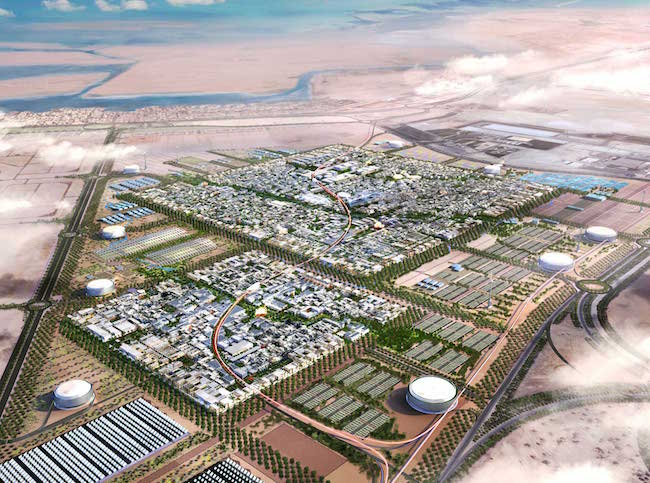
\includegraphics[width=70mm]{Masdar.jpg}
	\caption{マスダール・シティの完成イメージ \protect \footnotemark}
	\label{Masdar}
	\end{figure}
	\footnotetext{出典:Masdar社}
	このプロジェクトでは道路交通は自動運転車のみで構成される予定である。住民が任意の時刻に自動運転車に乗降し都市空間内を移動することを想定しているため,大量の車両の配備が必要となる。道路上の車両密度が高くなるため,渋滞やデッドロックが発生することが想定される。したがって,個々の車両だけではなく,自動運転車群が効率的に走行するアルゴリズムが必要となる。
	
	本研究では群制御アルゴリズムが安全性に関わる衝突回避やデッドロック回避,効率性に関わる時間制約などの性質を満たすかどうかを検証する手法を提案する。
	
	自動運転車の群制御アルゴリズムを形式的に記述し,モデル検査を用いて,性質を検証する。モデル検査は,システム上で起こり得る状態を網羅的に調べることにより設計の誤りを発見する自動検証手法の一種である。モデル検査手法は,システムの振る舞いの設計,および検証したい性質をそれぞれモデル化し,ツールを用いて,システムが性質を満たしているかを調べる。本研究では,時間オートマトンによる時間制約検証が行えるモデル検査ツールUPPAAL\cite{u1}を採用する。
\section{モデル検査}
	モデル検査は,システム上で起こり得る状態を網羅的に調べることにより設計の誤りを発見する自動検証手法の一種である。モデル検査手法は,システムの振る舞いの設計,および検証したい性質をそれぞれモデル化し,ツールを用いて,システムが性質を満たしているかを調べる。
	
	モデル検査において,システムの動作を表現するシステムモデルを作成する必要がある。ソフトウェア開発のどの段階でモデル検査を活用したいか,もしくは,何をどの程度検証したいかによって,どのような情報をもとにどのようにシステムモデルを作成するかが変わってくる。専用のシステムモデルを入力とするモデル検査を設計モデル検査,ソースプログラムを入力とするモデル検査をプログラムモデル検査と呼ぶ。これらのモデル検査がソフトウェア開発の流れの中での活用例を図\ref{develP}に示す。図\ref{develP}にはソフトウェアの品質向上のために行われる手順である設計レビュー,コードレビュー,およびテストも挙げた。設計モデル検査は設計レビューを,プログラムモデル検査はコードレビューをそれぞれ補完する位置付けである。
\section{群制御アルゴリズムのモデル化と検証}
UPPAALを用いて交差点を通過する1台の自動運転車の挙動をモデル化する。交差点は2車線対面通行で右折用レーンはなく,信号もない交差点とする。3.1節では時間は扱わず,任意の方向へ進む車両をモデル化する。3.2節では時間に関する条件を用いることで,交差点通過時間を記述する。3.3節では,全ての車両が交差点を通過するのに掛かる最小時間を検証する。	
\section{時間制約のない進行方向を固定しない交差点}
	本節では,経路選択をして交差点を通過する車両のモデルを作成する。信号のない交差点を無秩序に通過すると衝突などが起きる可能性がある。したがって今回は交差点に使用権というものを設定し,交差点を通過するにはこの使用権が取得できた車両が通過できることとする。
	
	\begin{figure}[htbp]
	\centering
	\includegraphics[width=70mm]{IntersectionM.png}
	\caption{交差点における使用権の鍵の組み合わせモデル}
	\label{IM}
	\end{figure}
	交差点に5つの鍵を設定し,その組み合わせで交差点を通過可能とする。図\ref{IM}は5つの鍵を用いた交差点の車両の進行モデルである。図上からの進入に対して,直進,右折,左折の選択肢があり,直進は鍵a,bを,右折は鍵aのみを,左折は鍵a,c,crossをそれぞれ取得する。該当の鍵を取得可能な時,その進行方向へ進入可能となる。図\ref{IM} を基にして,1台の車両の交差点通過を表すオートマトンを作成する。

	\subsection{時間オートマトンの作成}	
	図\ref{IB}は初期状態Startから交差点に進入し,通過後Startに戻ることで,上下左右の全ての方向から直進,右折,左折を非決定的に選択することを繰り返す1台の車両のオートマトンである。Startから交差点進入前状態rightOverに遷移したとき,車両は,直進,左折,右折の3つの選択肢がある。直進するときは,交差点通過中状態a4への遷移可能条件として大域変数a==0かつ,b==0すなわち使用されていないとき,遷移時にa=1とb=1として使用権を取得し,b4への遷移時にa=0として使用権の一部を解放する。そして,b4から交差点通過後状態UnderFへの遷移時にb=0としてもう1つの使用権も解放する。右折するときは,通過中状態a1への遷移可能条件をa==0とし,遷移時にa=0と更新し,使用権を取得する。通過後状態RightFへの遷移時にa=0として使用権を解放しStartに戻る。左折するときは,通過中状態a3への遷移条件をa==0かつ,c==0かつ,cross==0とし,遷移時に3変数を1に更新して使用権を取得する。通過中状態c3への遷移時にa=0として鍵aを解放し,c3から通過後状態LeftFへの遷移時に使用権を解放し,Startに戻る。以上の遷移を交差点に進入する4方向についてすべて記述する。
	\begin{figure}[htbp]
	\centering
	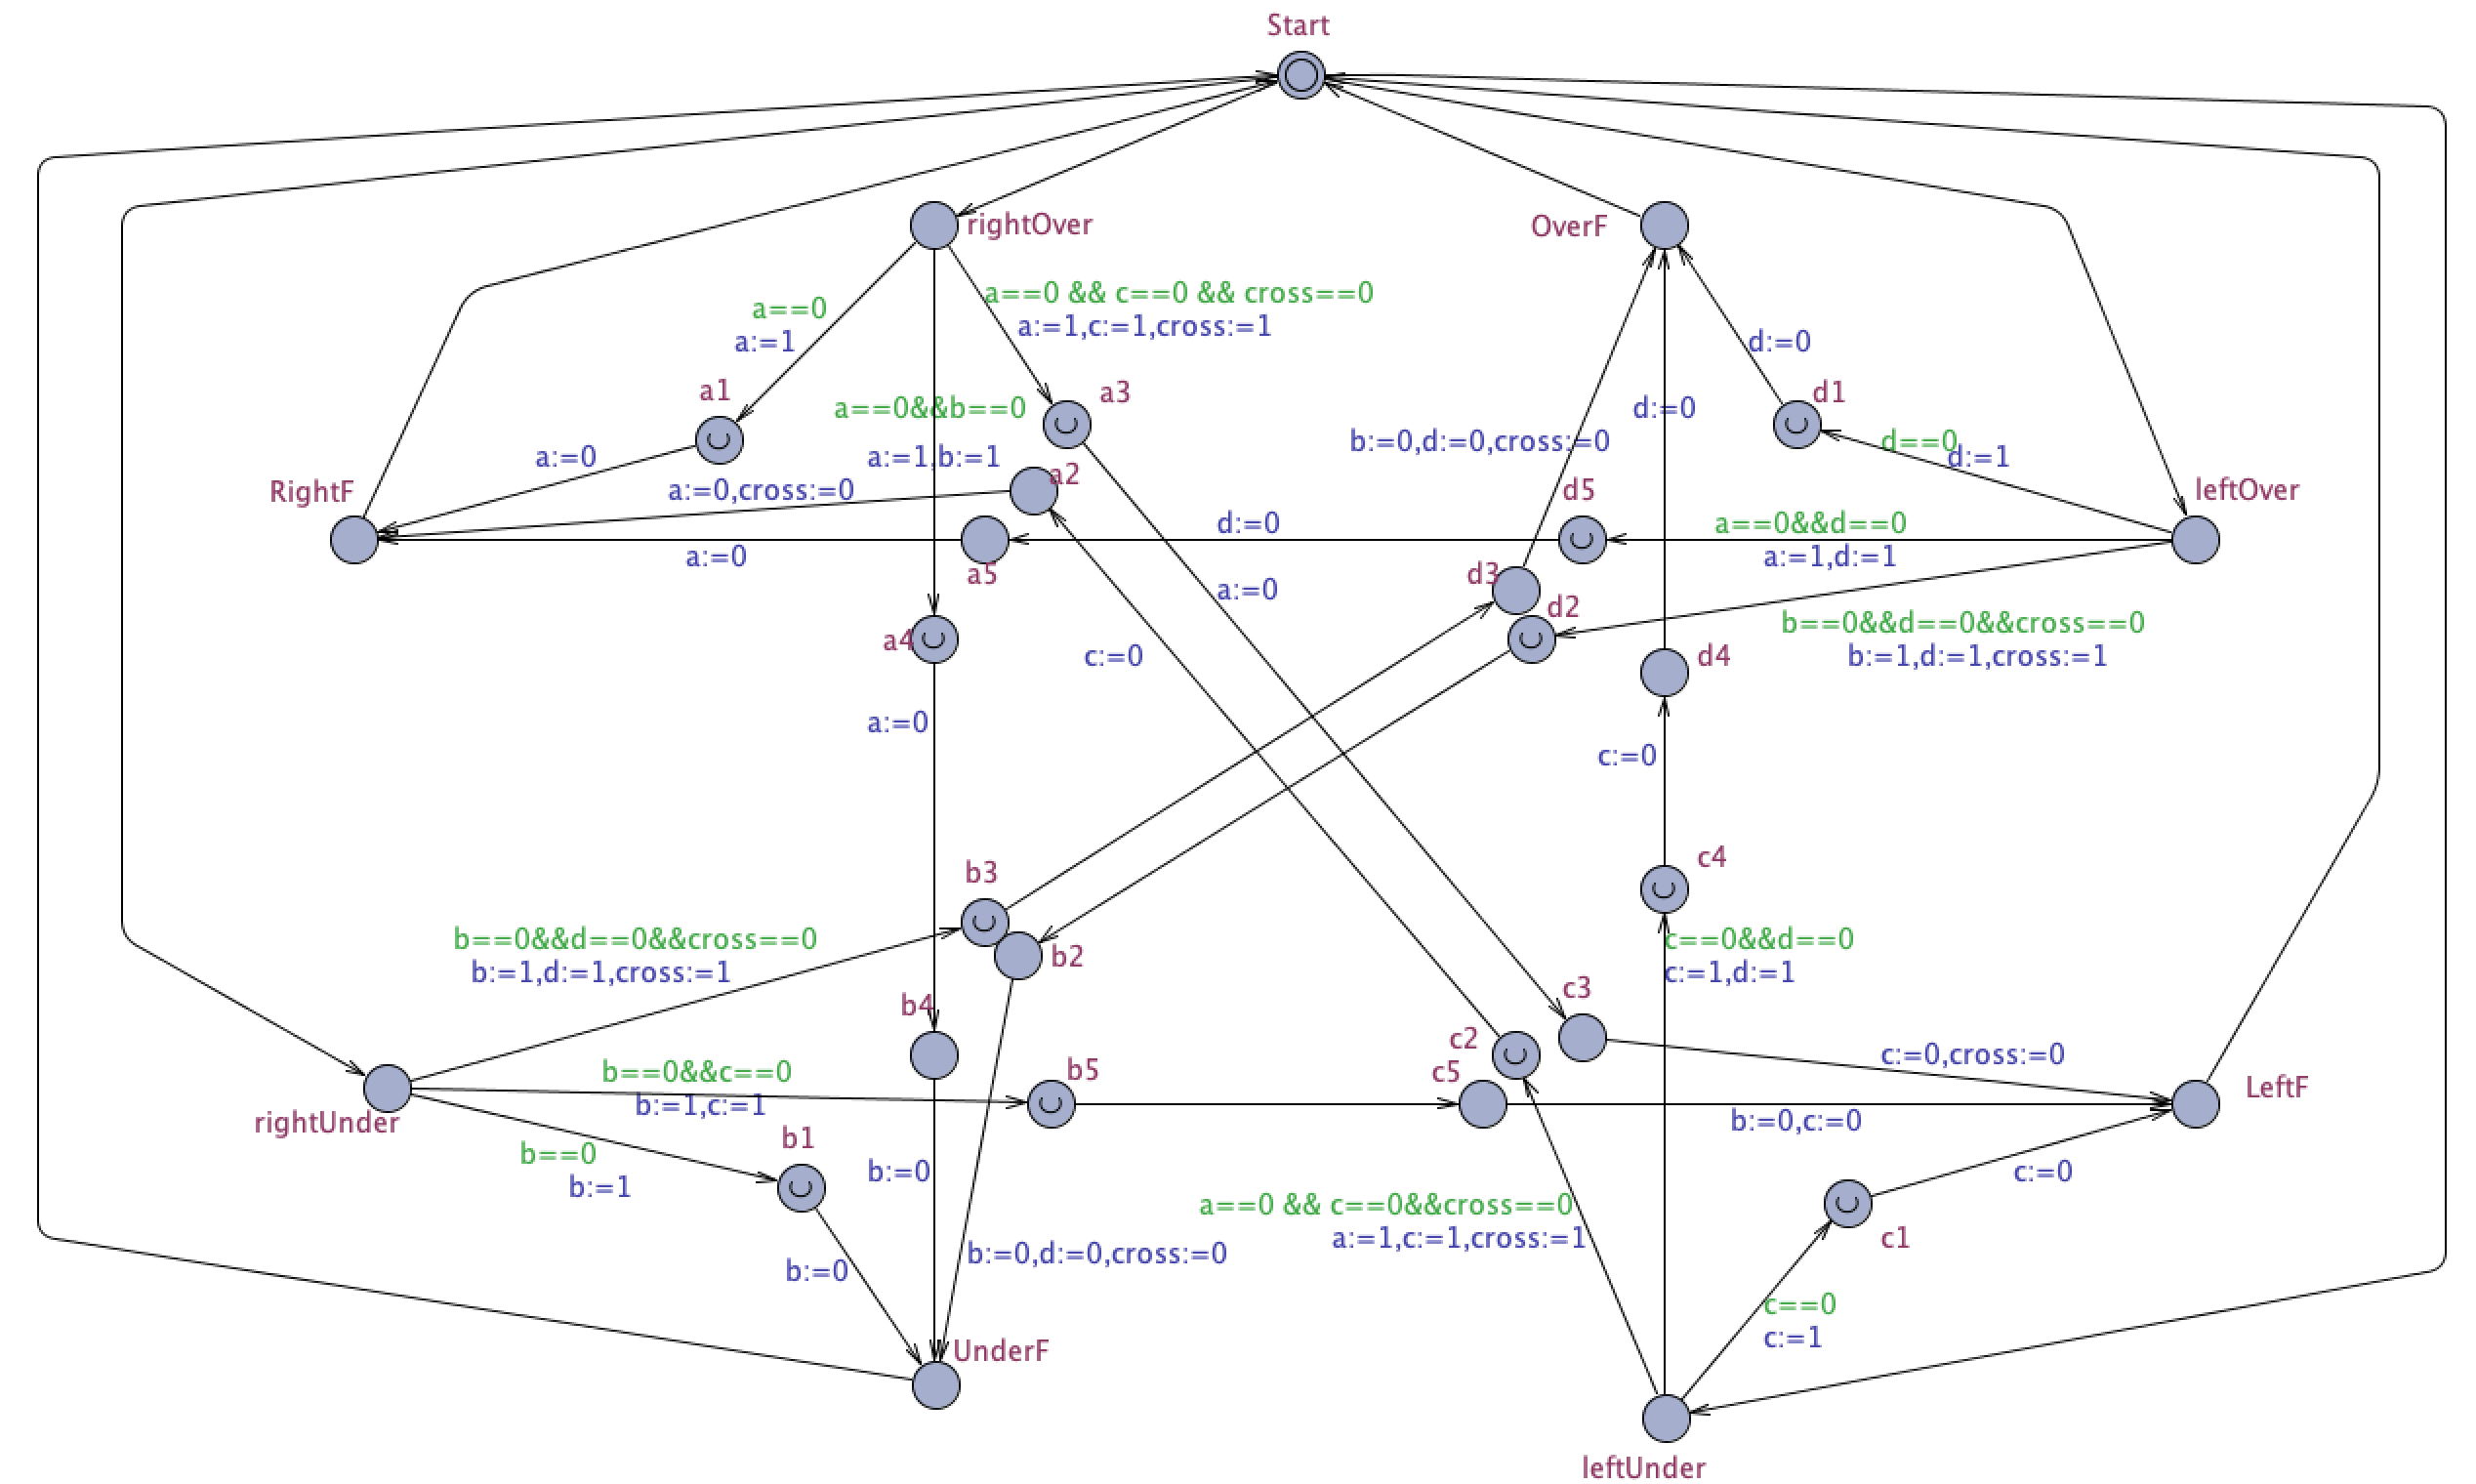
\includegraphics[width=70mm]{IntersectionBig.png}
	\caption{進行方向を固定しない交差点の時間オートマトン}
	\label{IB}
	\end{figure}
	\begin{figure}[htbp]
	\centering
	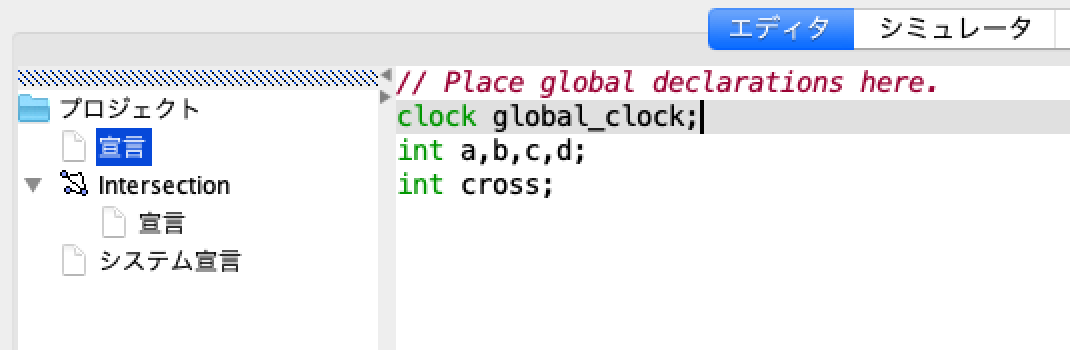
\includegraphics[width=70mm]{IBSimuGD.png}
	\caption{時間制約のない交差点の時間オートマトンの大域情報}
	\label{IBSi}
	\end{figure}
	\subsection{シミュレーション}
	前節で作成した時間オートマトンのインスタンスを2つ宣言し,シミュレーションを行う。図\ref{IBSi}では,Car1 はleftOverから右折して交差点を通過中状態で,Car2はrightOverで交差点進入前状態である。このとき大域変数は図\ref{IBSGS}となっている。したがって,Car2は直進右左折それも選択可能となっている(図\ref{IBST})。
	\begin{figure}[htbp]
	\centering
	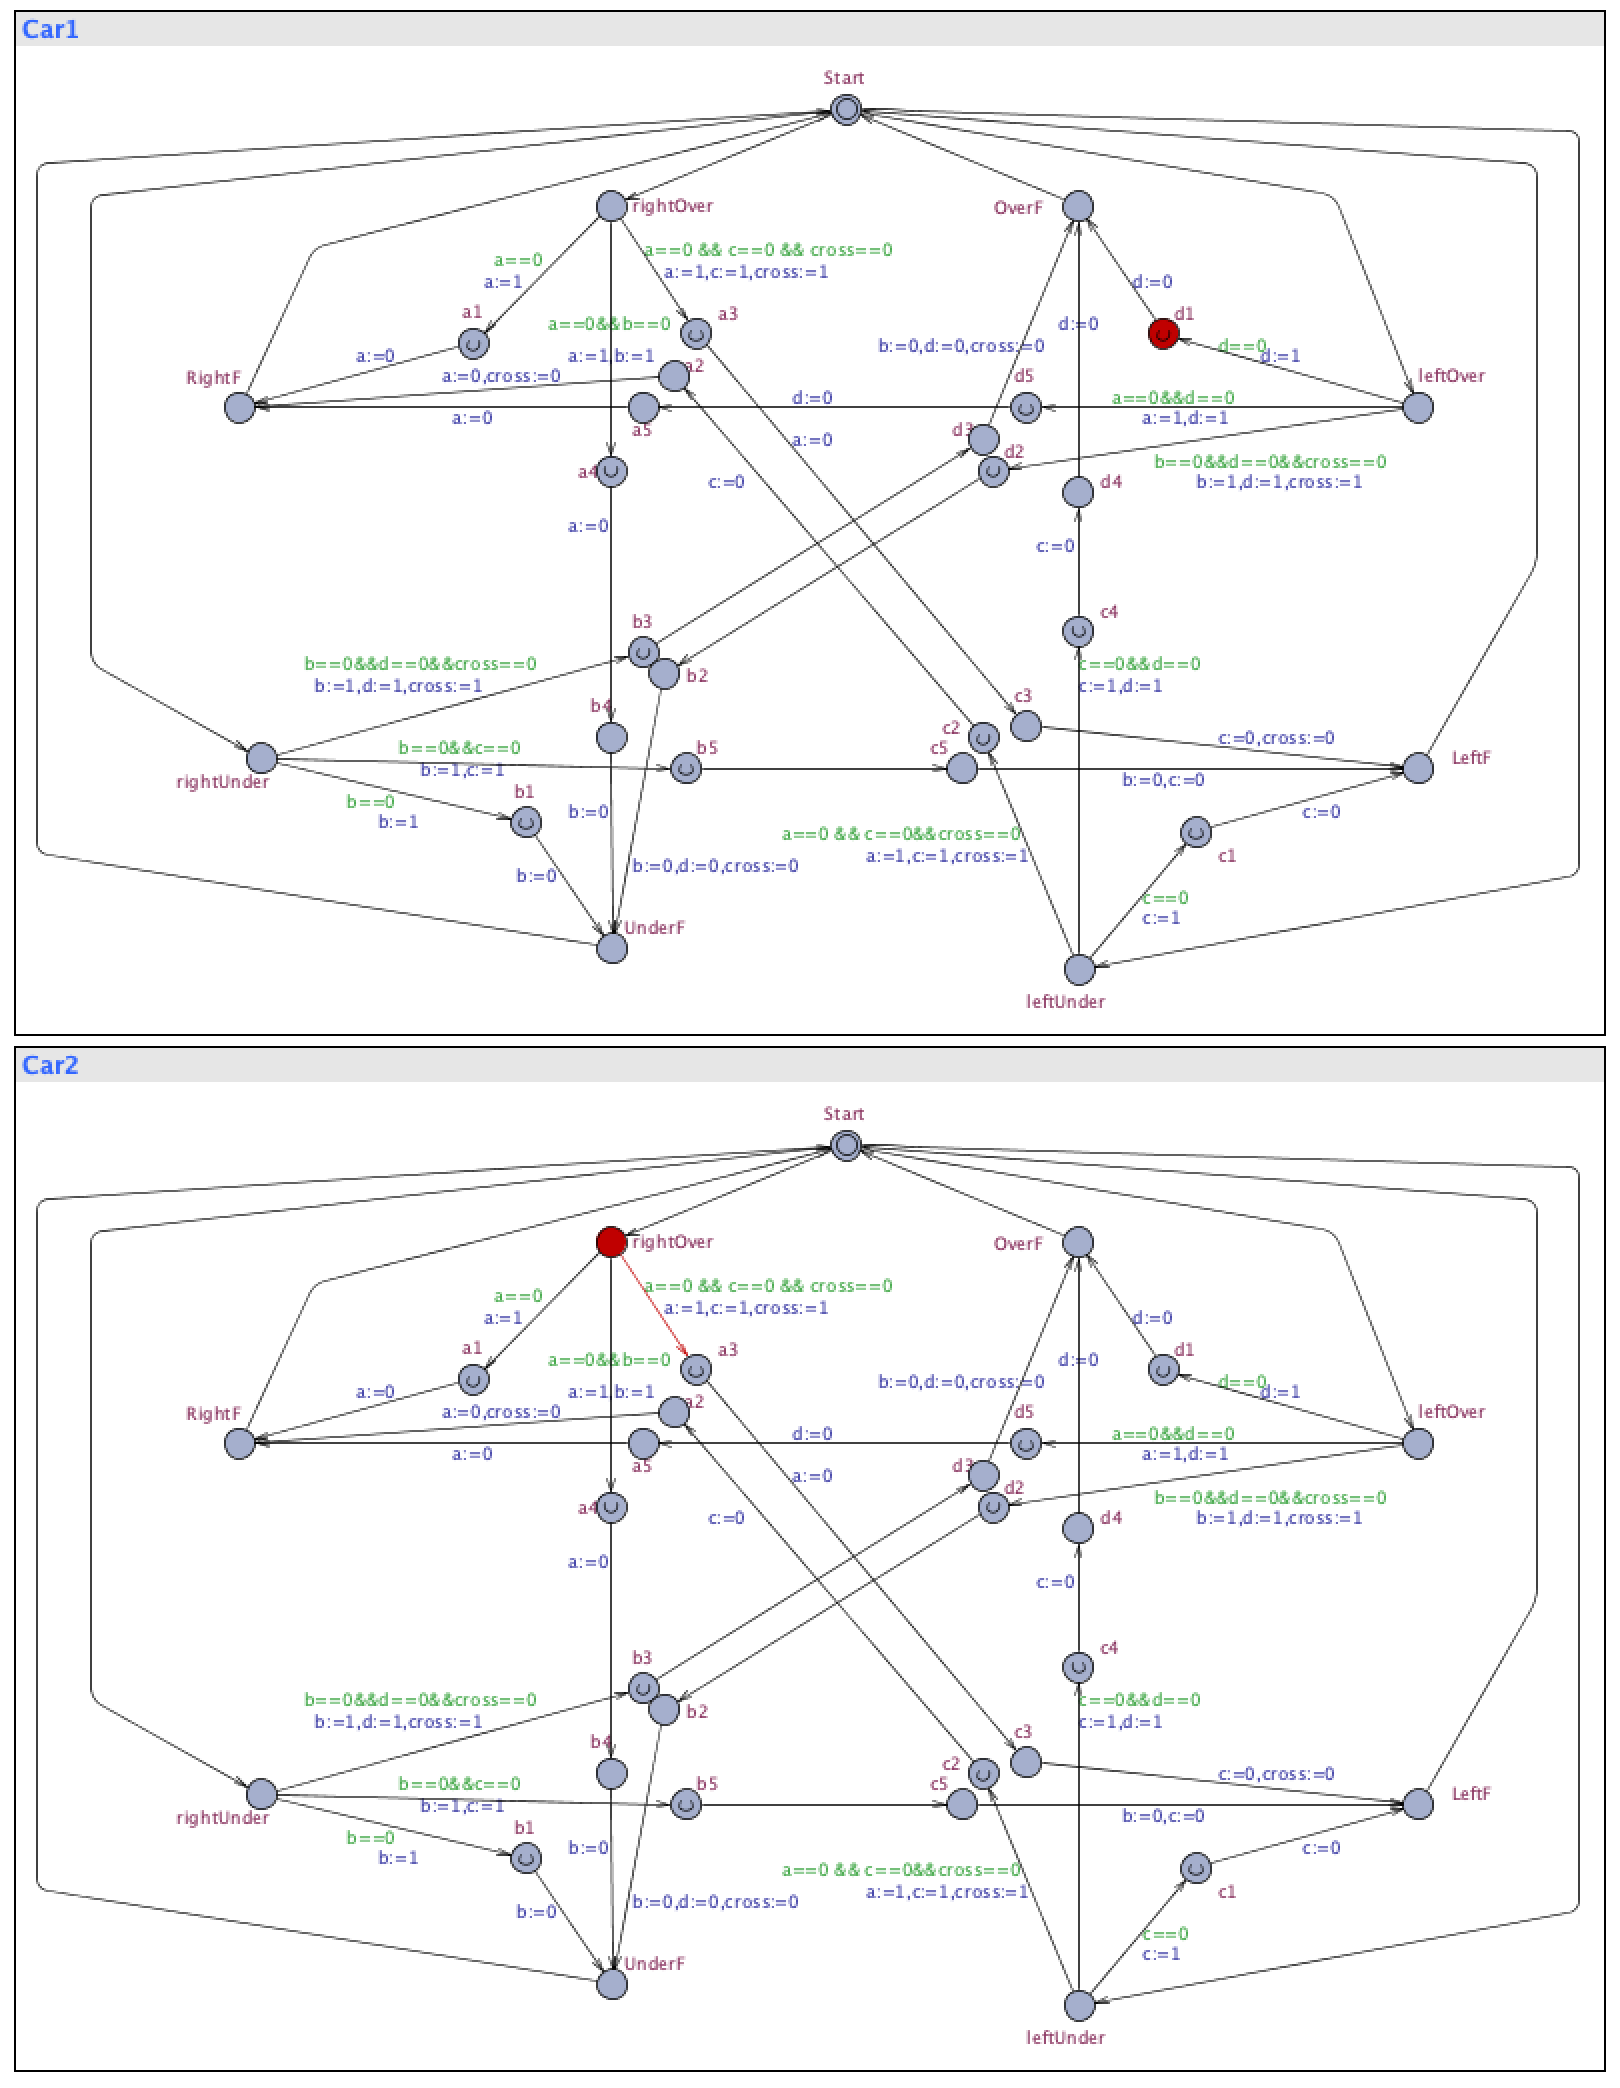
\includegraphics[width=65mm]{IBSimu.png}
	\caption{時間制約のない交差点の時間オートマトン}
	\label{IBSi}
	\end{figure}
	\begin{figure}[htbp]
	\centering
	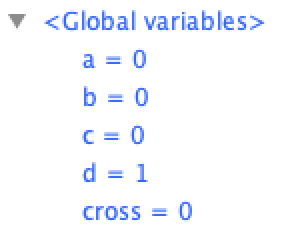
\includegraphics[width=50mm]{IBSimuGS.png}
	\caption{時間制約のない交差点の時間オートマトンの大域変数値}
	\label{IBSGS}
	\end{figure}
	\begin{figure}[htbp]
	\centering
	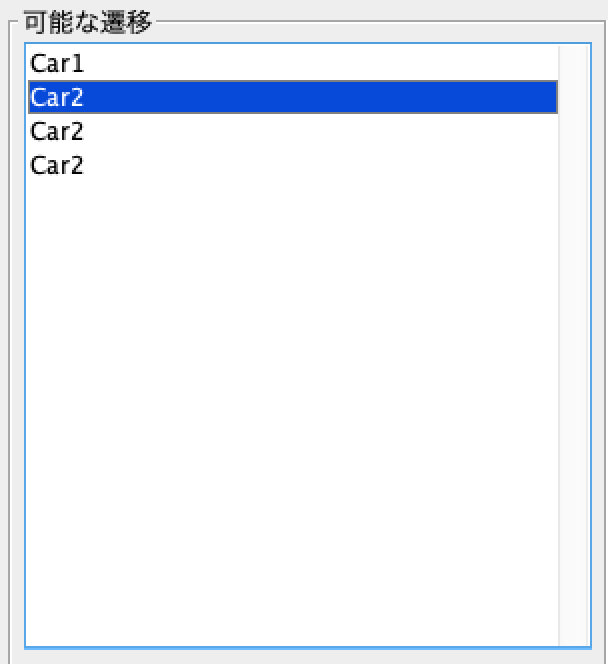
\includegraphics[width=80mm]{IBSimuTra.png}
	\caption{時間制約のない交差点の時間オートマトンの実行可能遷移一覧}
	\label{IBST}
	\end{figure}
	\subsection{モデル検査}
	UPPAALでは,どれだけ時間が経過しても,いずれのプロセスも遷移できないことをデッドロックという。本モデルでデッドロックが起きないか検証する。本例題におけるデッドロックは同じ鍵を同時に使うことや,Startに戻ってこれないことを指す。すべての実行列で常にデッドロックにならないことを表す検証式は次のように記述される:
	\[
	\mbox{\tt{A[] not deadlock}}
	\]
	検証結果は図\ref{IBC6}のように示される。
	
	プロセスの車両インスタンスを1から6まで1ずつ増やしながらデッドロック検証を行った。表\ref{a}は車両の台数に対する検証にかかった時間である。図\ref{IVT}はそれをグラフ化したものである。
	\begin{figure}[htbp]
	\centering
	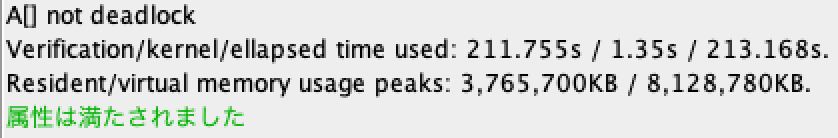
\includegraphics[width=70mm]{InterBigCar6.png}
	\caption{進行方向を固定しない交差点のデッドロック検証結果}
	\label{IBC6}
	\end{figure}
	
	\begin{table}[htb]
	\centering
	\caption{車両の台数とデッドロック検証にかかる時間}
	\label{a}
	 \begin{tabular}{|c|r|} \hline
	    車両の台数 & 検証時間(s)  \\ \hline
	   1& 0.00  \\ \hline
	   2 & 0.004 \\ \hline
	   3 & 0.068 \\ \hline
	   4 & 0.808 \\ \hline
	   5 & 10.873 \\ \hline
	   6 & 211.755\\ \hline
	 \end{tabular}
	 \label{testcase}
	\end{table}
	
	\begin{figure}[htbp]
	\centering
	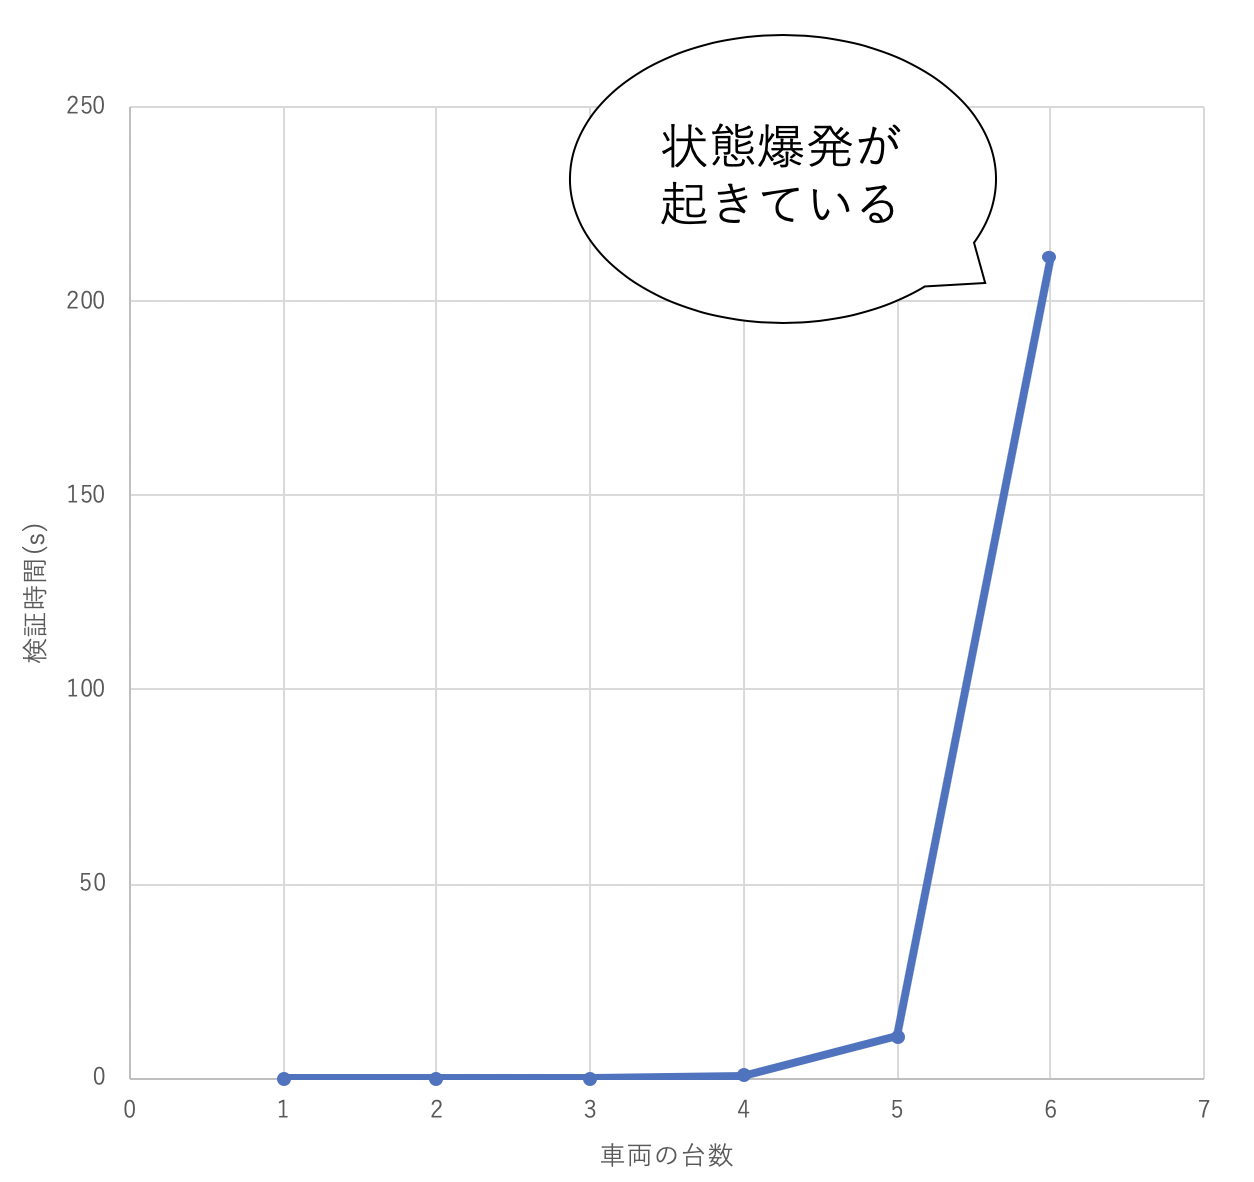
\includegraphics[width=70mm]{IntersectionVerificationTime.png}
	\caption{車両の台数と検証にかかる時間の関係}
	\label{IVT}
	\end{figure}

	
	\section{時間制約を用いる進行方向を固定する交差点}
	本節では,交差点に進入する車両の進行方向を固定して,時間オートマトン\cite{u3}を作成する。車両1台の挙動は,交差点進入前,交差点通過中,交差点通過後の3つの状態で記述する。交差点進入前に交差点の使用権を取得し,通過後に使用権を解放する。遷移可能条件と状態不変条件に時間に関する条件を与えることによって,通過にかかる時間や使用権を何秒前に取得しなければならないかを記述できる。
	\subsection{一方通行の2車線で構成される交差点モデル}
	\begin{figure}[htbp]
	\centering
	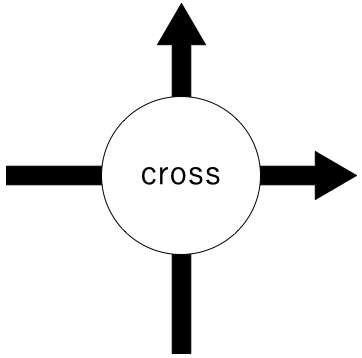
\includegraphics[width=60mm]{SimplePerpendicular.png}
	\caption{交差点の使用権}
	\label{SimpleP}
	\end{figure}
	一方通行の交差点で互いの進行方向が交わる時,交差点を図\ref{SimpleP}のようにモデル化する。crossは交差点の使用権を表現しており,使用権を取得できた車両が交差点を通過するモデルである。
	\subsubsection{時間オートンマトンの作成}
	交差点に直進する車両2台の進行方向が互いに交差するとき,衝突回避するためには交差点に同時に進入するのは1台までにする。交差点進入時に使用権を取得する車両の時間オートマトンを作成する(図\ref{Perpendicular})。respawnは車両の初期状態かつ,任意の時刻に車両が発生する状態である。BeforeEnterは車両の交差点進入前の状態である。crossAreaは交差点通過中の状態である。Passedは交差点通過後の状態である。respawnからBeforeEnterへの遷移可能条件のcross==0は交差点の使用権が未獲得であることを示しており,遷移時にcross==1と更新して交差点使用権を獲得する。同時にタイマーであるlocal\_clockを0にして,BeforeEnterの時間を測定する。BeforeEnterからcrossAreaの遷移でも同様にし,交差点手前の約5秒から10秒前までに使用権を獲得し,交差点通過に2秒から5秒弱かかるということが記述されている。
	
	\begin{figure}[htbp]
	\centering
	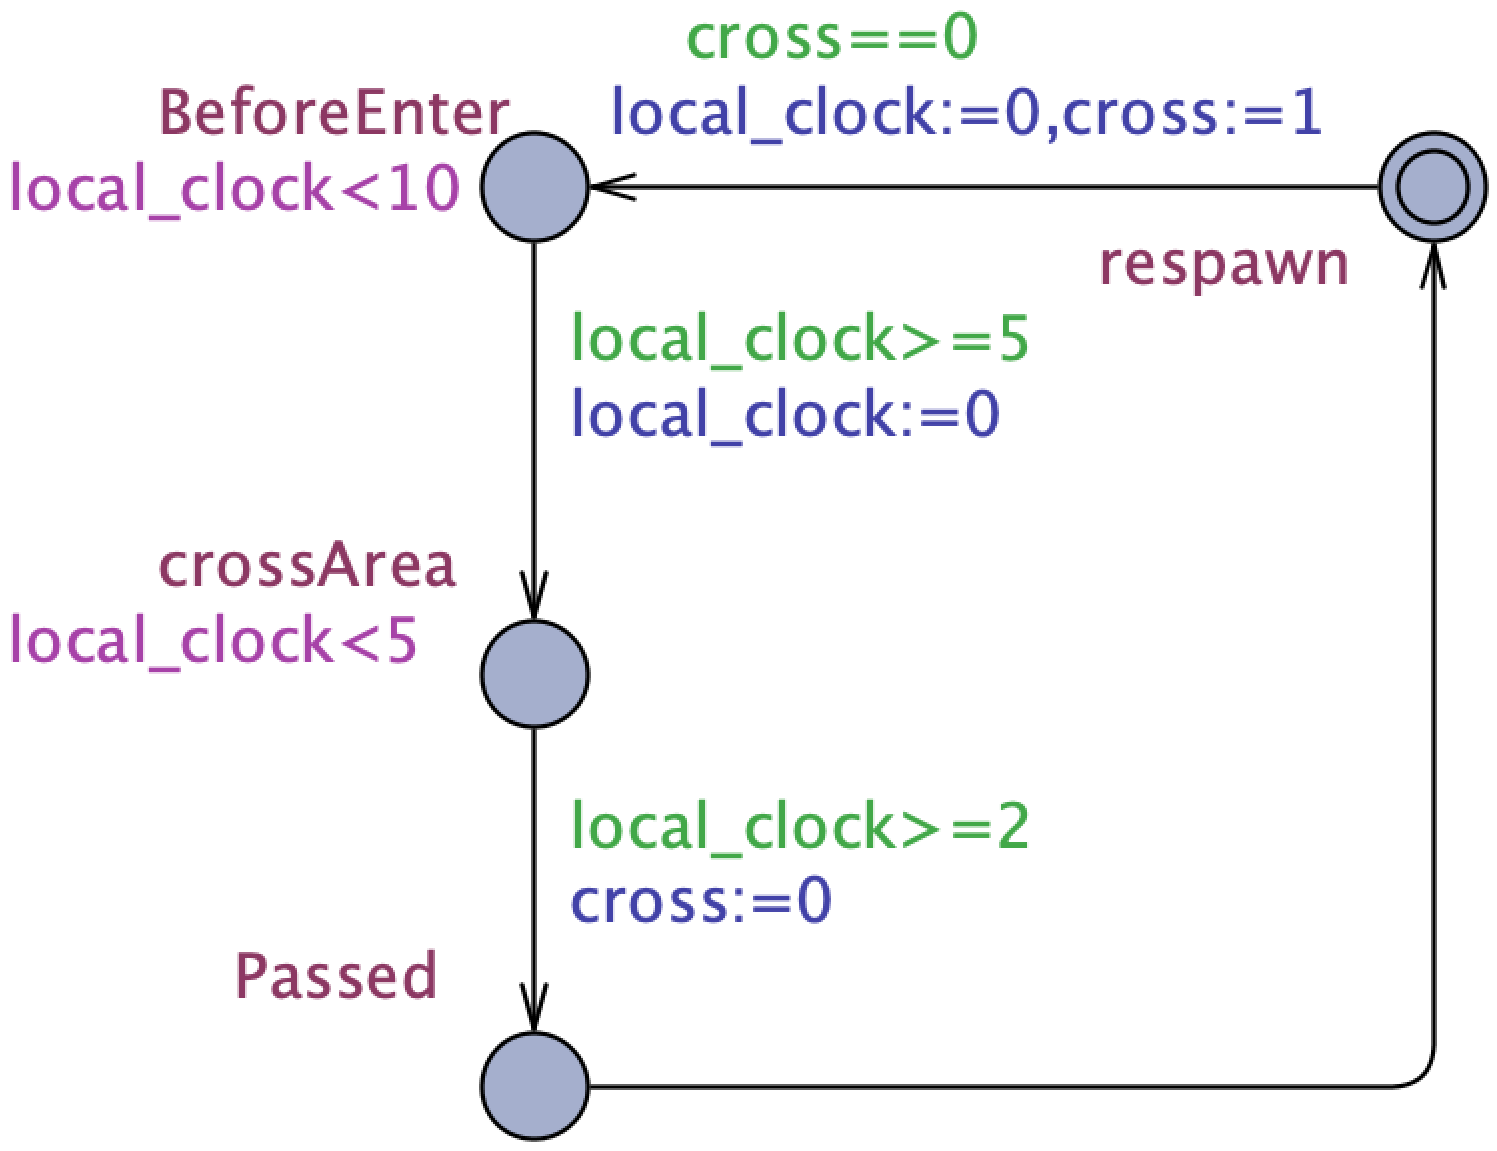
\includegraphics[width=65mm]{Perpendicular.png}
	\caption{交差点進入時に使用権を取得する車両1台の時間オートマトン}
	\label{Perpendicular}
	\end{figure}
	
	\subsubsection{シミュレーション}
	
	図\ref{PerpendicularS}は,前節で定義したテンプレートから生成された2つのインスタンスが合成された時間オートマトンに対するシミュレーションのスクリーンショットである。左のプロセスverticalを縦方向に直進してるとし,右のプロセスhorizonを横方向に直進しているとする。現在状態はverticalが交差点の使用権を獲得し,進入前状態で,horizonが交差点通過後の状態である。
	\begin{figure}[htbp]
	\centering
	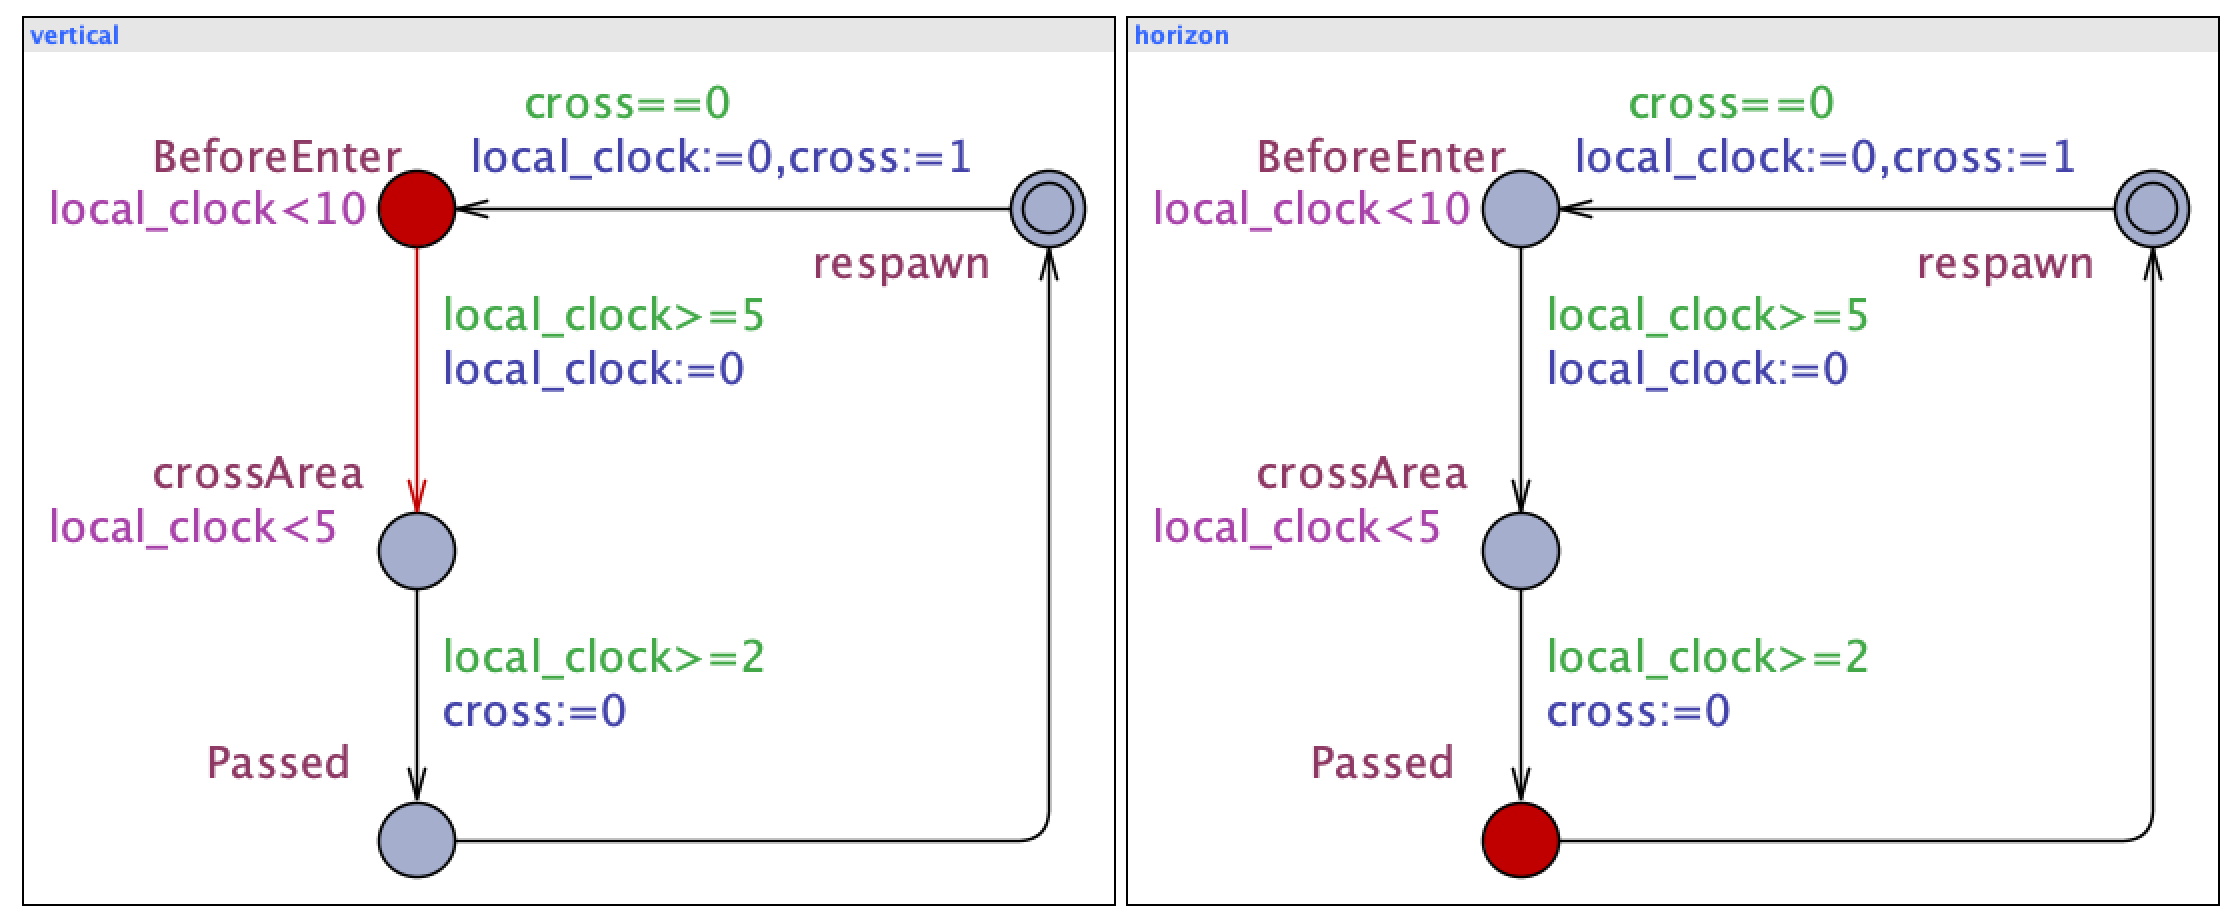
\includegraphics[width=70mm]{PerpendicularSimu.png}
	\caption{垂直に交差点に進入する車両の時間オートマトンの合成}
	\label{PerpendicularS}
	\end{figure}
	
	\subsubsection{モデル検査}
	このモデルでデッドロック検証を行った結果を図\ref{PerV}に示す。
	\begin{figure}[htbp]
	\centering
	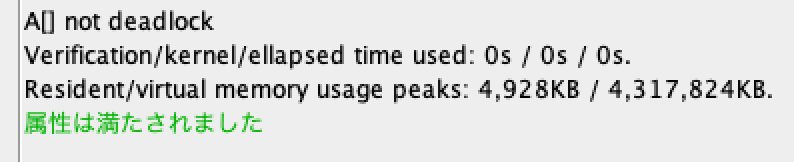
\includegraphics[width=70mm]{PerV.png}
	\caption{一方通行の2車線で構成される交差点のデッドロック検証結果}
	\label{PerV}
	\end{figure}
	
	\subsection{東西南北それぞれから交差点に直進する時間オートマトン}
	直進して交差点を通過する車両の進行方向に対して,他の車両の進行方向が垂直であったり,平行であったりする時の交差点の使用権の獲得方法を考える。前例では,crossが交差点の使用権そのものでそれの有無で進入を決定していたが,本例では,進行方向が平行となる場合は同時に進入可能としたい。したがって交差点の使用権を図\ref{oTWoL}に示すように4つの鍵の組み合わせで管理したい。例えば,西から東へ進行する車両はlock1とlock2を取得する。北から南へ進行する車両はlock2とlock4を取得しようとするが,既にlock2が取得されているためこの車両は交差点へ進入できない。一方で前者に対して,東から西へ進行する車両はlock3とlock4を取得できるため,交差点へ進入する。
	\begin{figure}[htbp]
	\centering
	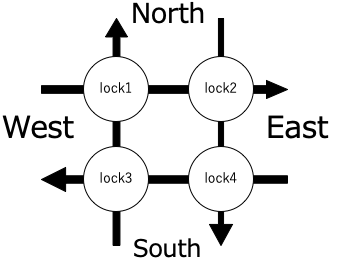
\includegraphics[width=70mm]{onTheWayofLock.png}
	\caption{交差点の使用権を管理する4つの鍵の組み合わせ}
	\label{oTWoL}
	\end{figure}
	\subsubsection{時間オートマトンの作成}
	使用権を4つの鍵で管理する交差点に直進する車両の時間オートマトンを作成する(図\ref{news})。遷移可能条件をパラメータ(L1,L2)で記述し,それぞれが取得する鍵に紐付けている。初期状態respawnから交差点進入前状態BeforeEnterへ遷移時にふたつの鍵L1とL2を1に更新して使用権を取得する。前例と同様にこのオートマトンも直進のみのため,タイマーであるlocal\_clockは同内容を記述している。交差点通過中状態crossAreaから交差点通過後状態Passedへの遷移時に鍵の解除としてL1==0とL2==0と記述した。
	\begin{figure}[htbp]
	\centering
	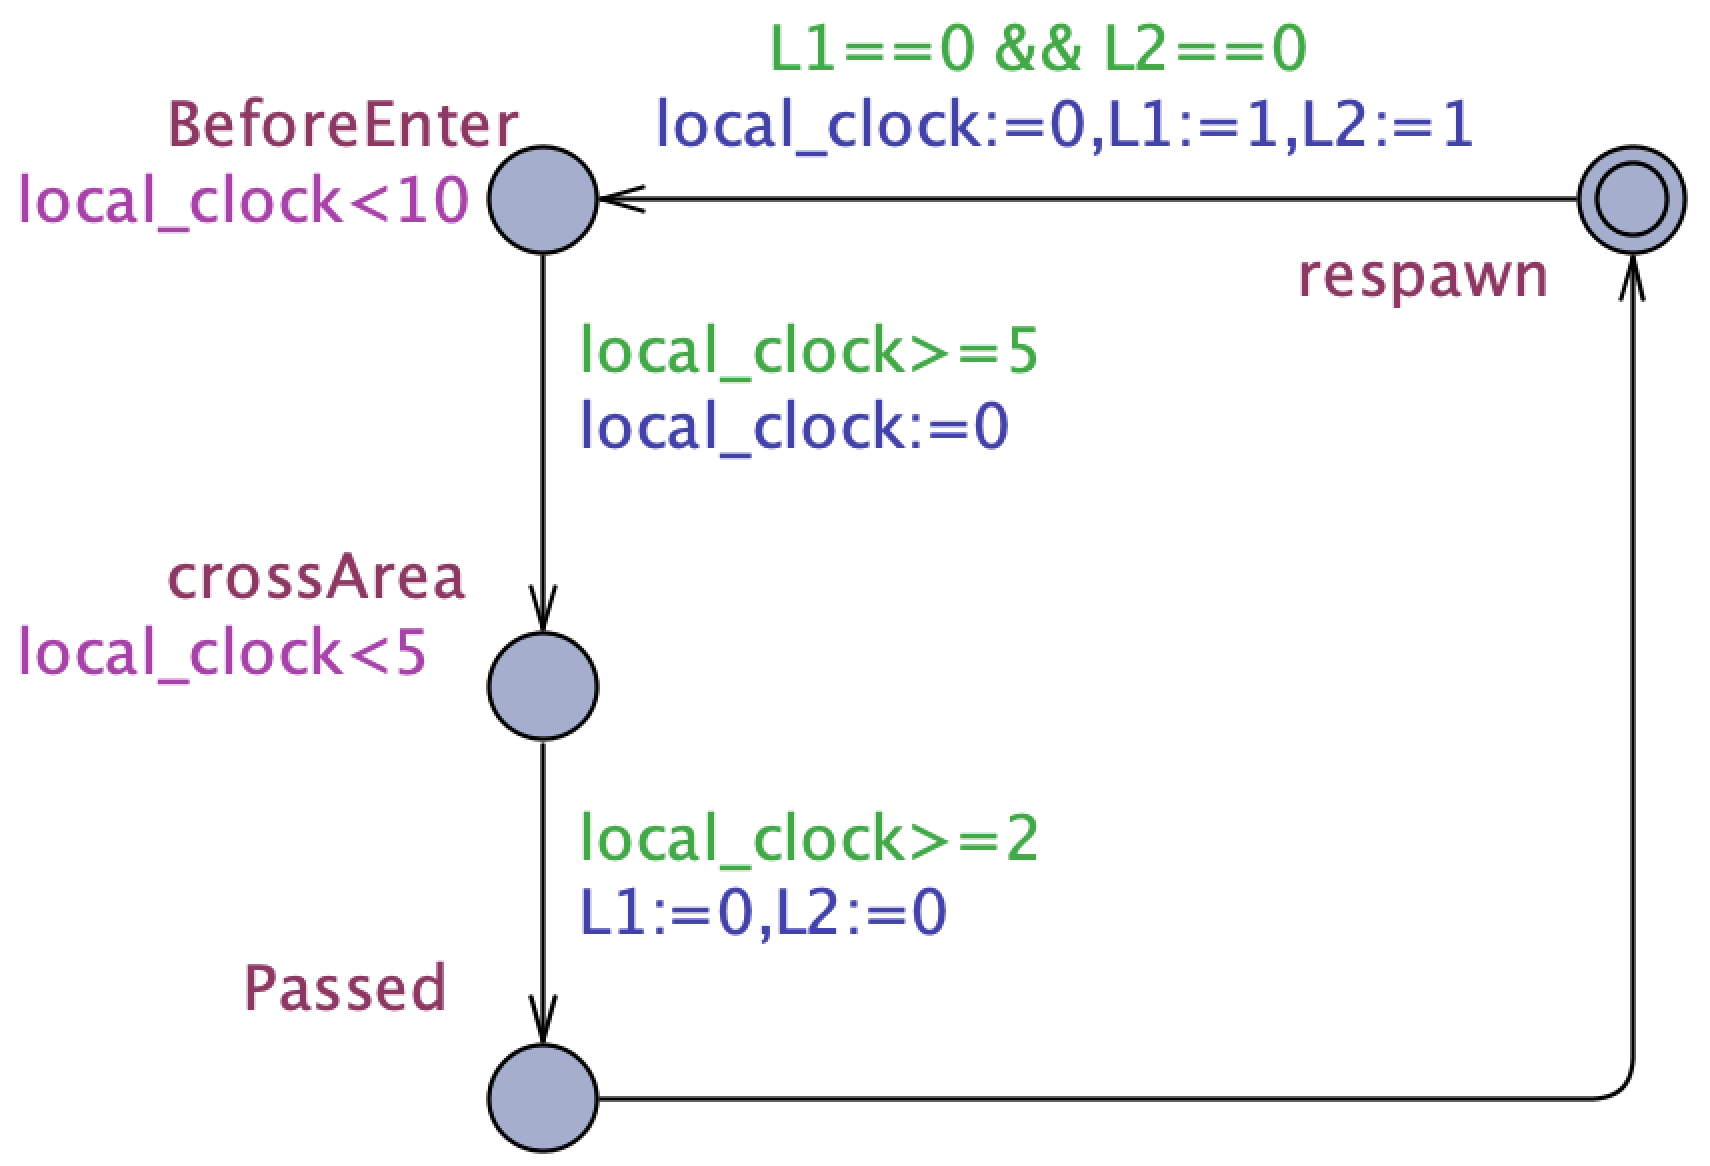
\includegraphics[width=70mm]{news.png}
	\caption{使用権を4つの鍵で管理する交差点に直進する車両の時間オートマトン}
	\label{news}
	\end{figure}
	\subsubsection{シミュレーション}
	北から南へ直進する車両をsn,南から北へ直進する車両をns,東から西へ直進する車両をew,西から東へ直進する車両をweとして,インスタンスの宣言をした(図\ref{newsSD})。図\ref{newsS}では,ewが交差点を交差点通過中で,lock3とlock4が取得されている。lock1とlock3を取得できたweが交差点進入前状態である。
	\begin{figure}[htbp]
	\centering
	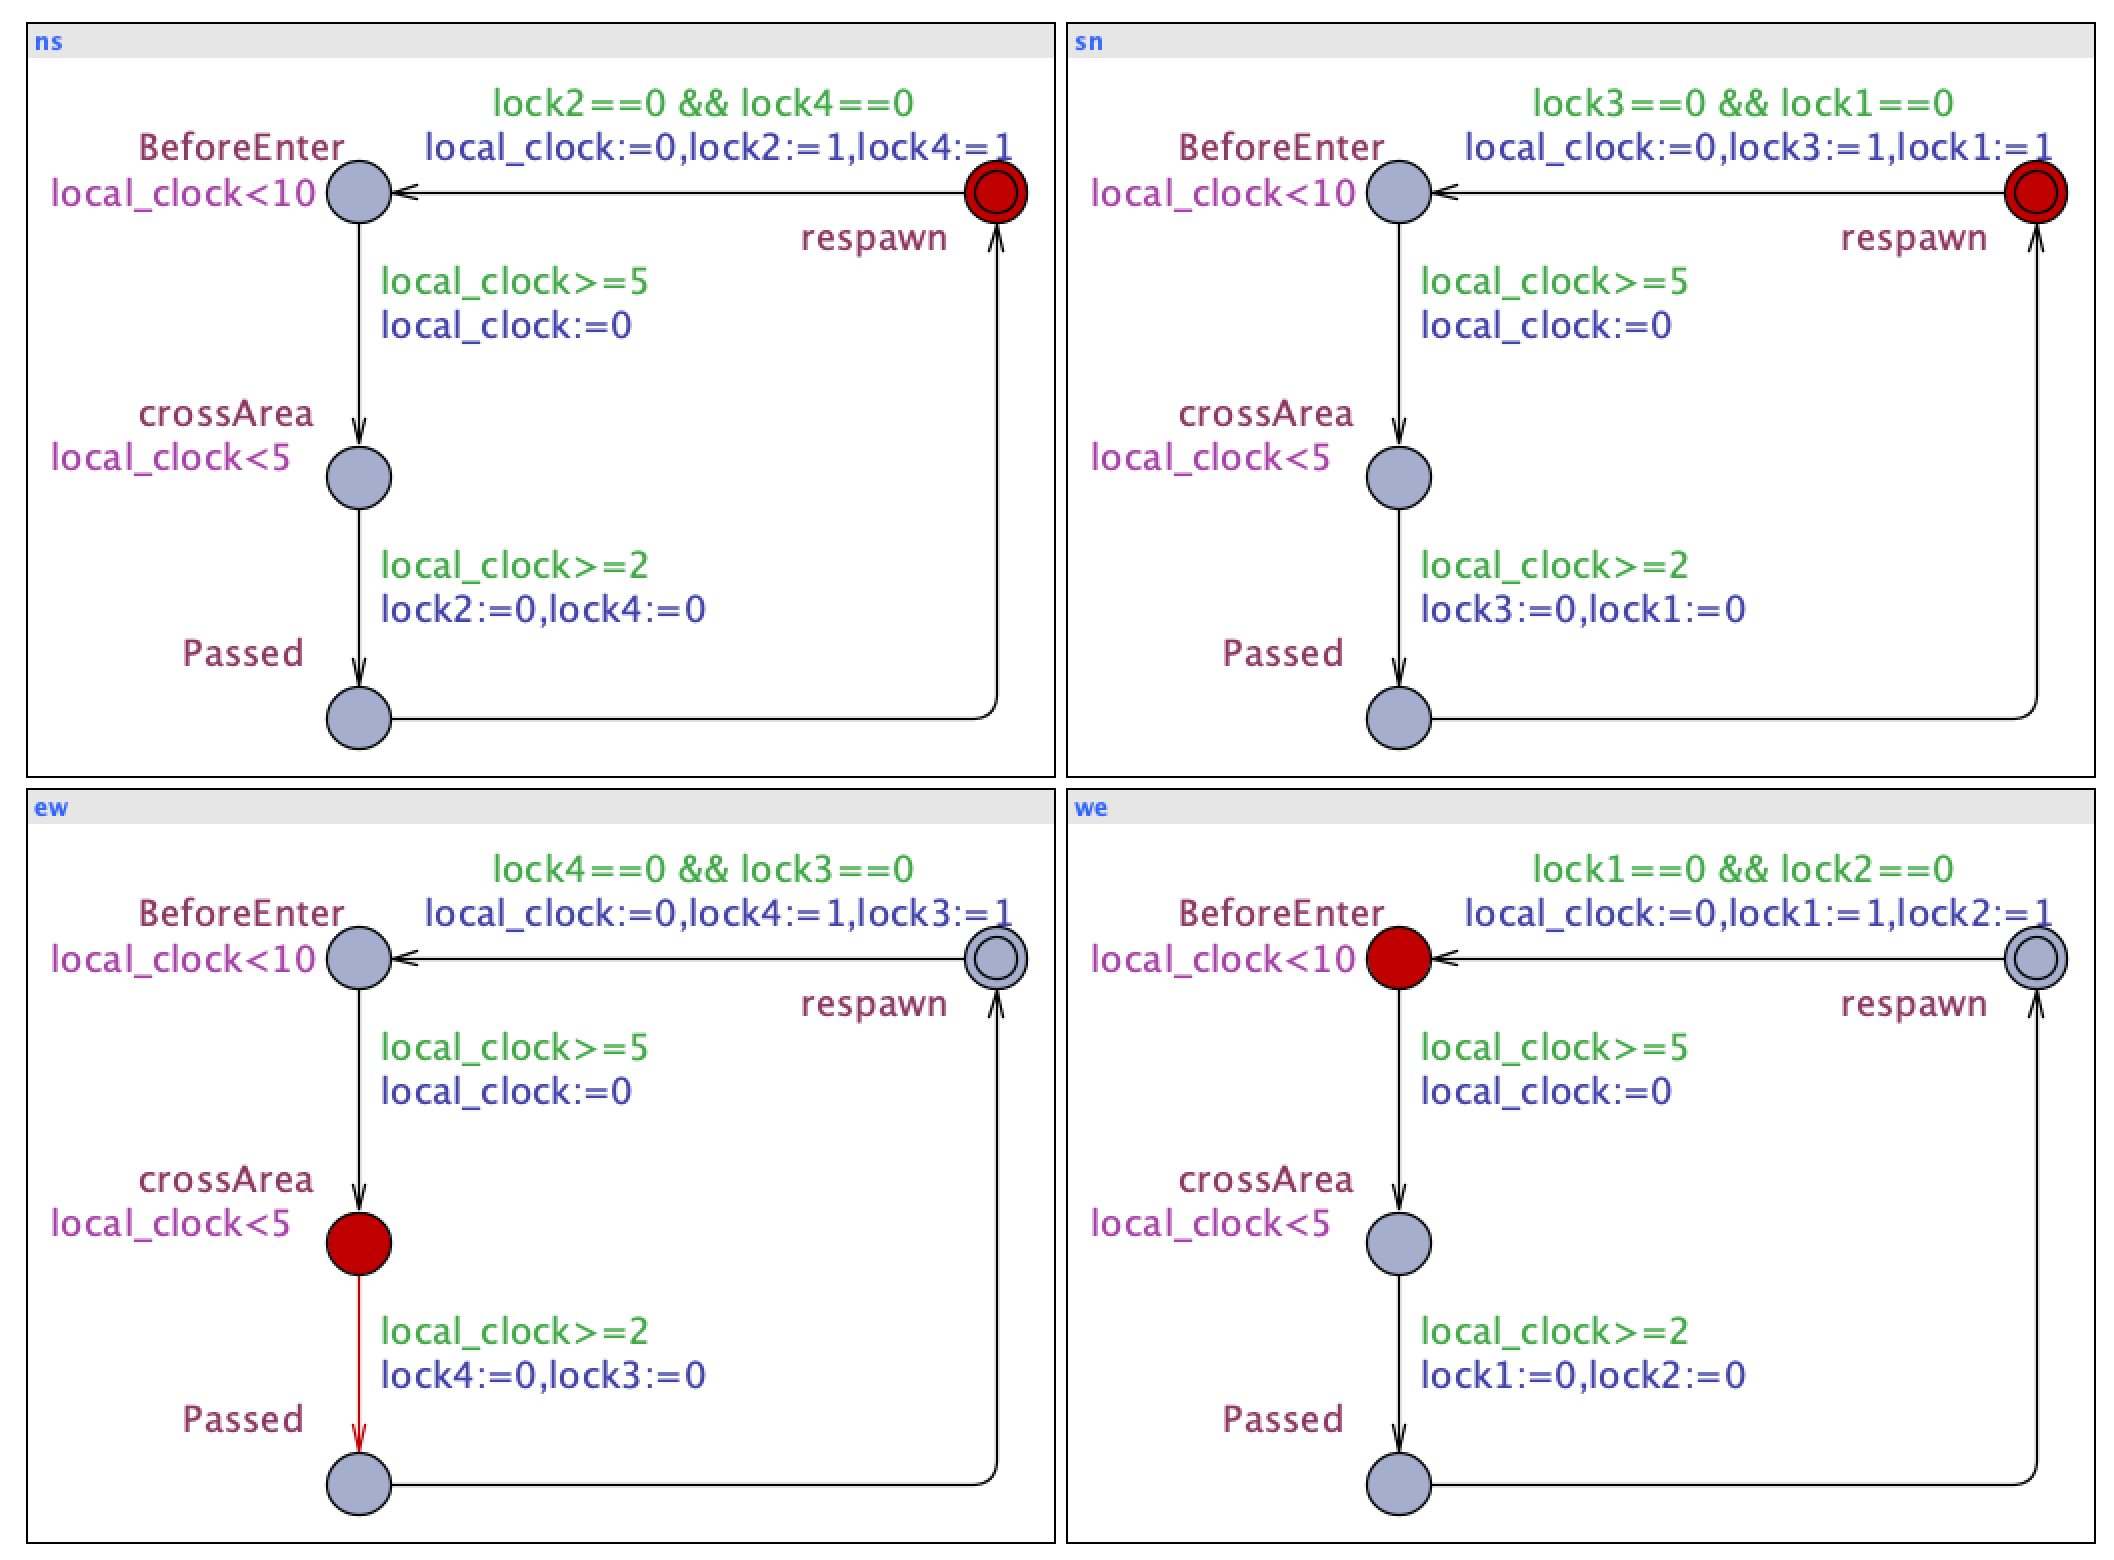
\includegraphics[width=70mm]{newsSimu.png}
	\caption{交差点に直進する車両の時間オートマトンの合成}
	\label{newsS}
	\end{figure}
	\begin{figure}[htbp]
	\centering
	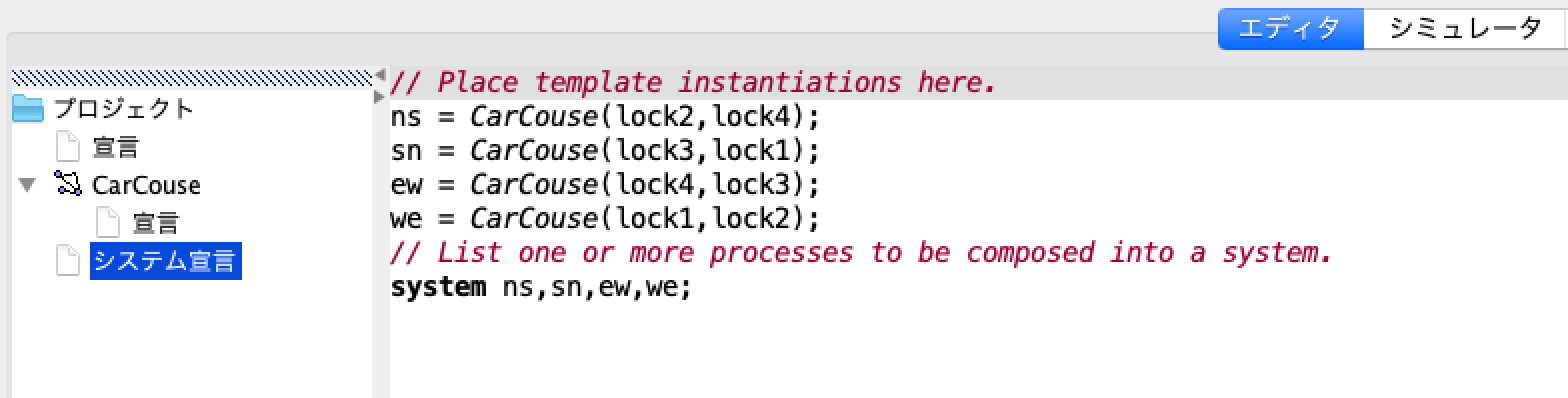
\includegraphics[width=70mm]{newsSD.png}
	\caption{4車両のシステム宣言}
	\label{newsSD}
	\end{figure}
	\subsubsection{モデル検査}
	デッドロック検証を行った結果を図\ref{newsV}に示す。
	\begin{figure}[htbp]
	\centering
	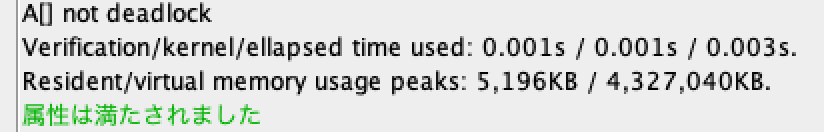
\includegraphics[width=70mm]{newsV.png}
	\caption{4車線で構成される交差点のデッドロック検証結果}
	\label{newsV}
	\end{figure}
	\subsection{交差点を直進・左折・右折する車両の時間オートマトン}
	交差点を直進する車両と左折する車両と右折する車両を考慮したモデルを考える。前述までとは違い,右折する場合もあるため,4つの鍵の組み合わせでは右折する車両同士での衝突が起こる可能性がある。したがって前述の4つの鍵に加えて,5つ目の鍵を右折用の鍵としてcrossを用意したモデルを考える。このモデルで同時通行可能な組み合わせの2つの例を図\ref{RL}と図\ref{4L}に示す。
	\subsubsection{時間オートマトンの作成}
	このモデルから時間オートマトンを作成する(図\ref{Simple})。鍵crossは3つ目のパラメータuseの値と照らし合わせる。パラメータuseは右折用の鍵を使用するかどうかを車両の固定情報として保持している。初期状態respawnから交差点進入前状態BeforeEnterへの遷移可能条件をパラメータL1,L2,右折用鍵crossが取得可能であることとした。また,左折時は,パラメータは2つあるが,取得する鍵は1つである。そのため,南から東へ右折する車両と,東から南へ左折する車両と,西から北へ左折する車両の3台が同時に交差点に進入可能となっている。
	\begin{figure}[htbp]
	\centering
	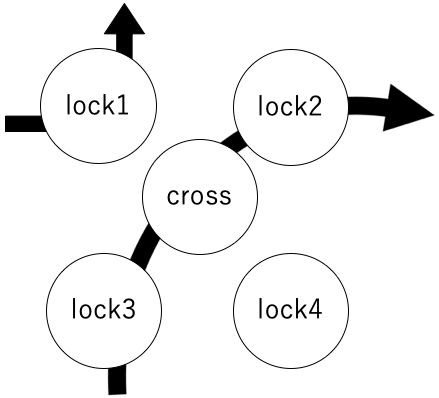
\includegraphics[width=70mm]{wn-se.png}
	\caption{使用権の取得例:右折と左折}
	\label{RL}
	\end{figure}
	\begin{figure}[htbp]
	\centering
	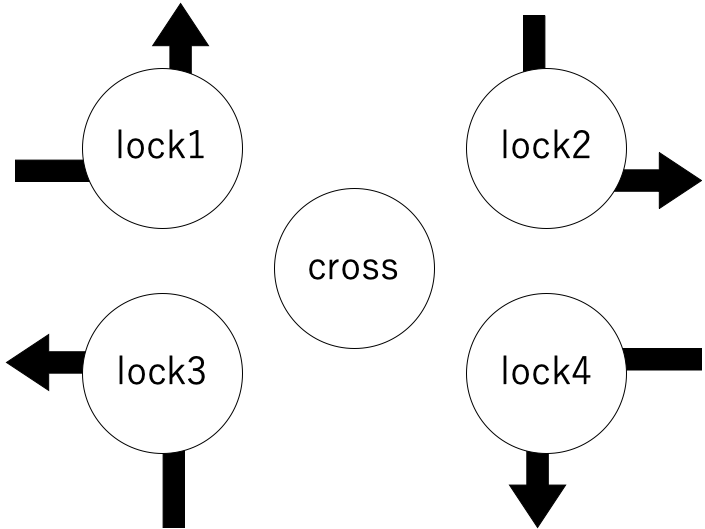
\includegraphics[width=65mm]{leftcouse.png}
	\caption{使用権の取得例:4台の左折}
	\label{4L}
	\end{figure}
	\subsubsection{シミュレーション}
	北から南へ直進する車両をsn,南から北へ直進する車両をns,東から西へ直進する車両をew,西から東へ直進する車両をwe,北から東へ左折する車両をne,南から西へ左折する車両をsw,東から南へ左折する車両をes,西から北へ左折する車両をwn,北から西へ右折する車両をsw,南から東へ右折する車両をse,東から北へ右折する車両をen,西から南へ右折する車両をwsとして,インスタンスの宣言をする(図\ref{SimpleSD})。上記の3台の車両が交差点に進入する例が図\ref{SimpleS}のように,右折するseが通過中状態crossAreaの時,左折するesも状態crossAreaで,もう一つのwnが状態BeforeEnterとなっている。
	\begin{figure}[htbp]
	\centering
	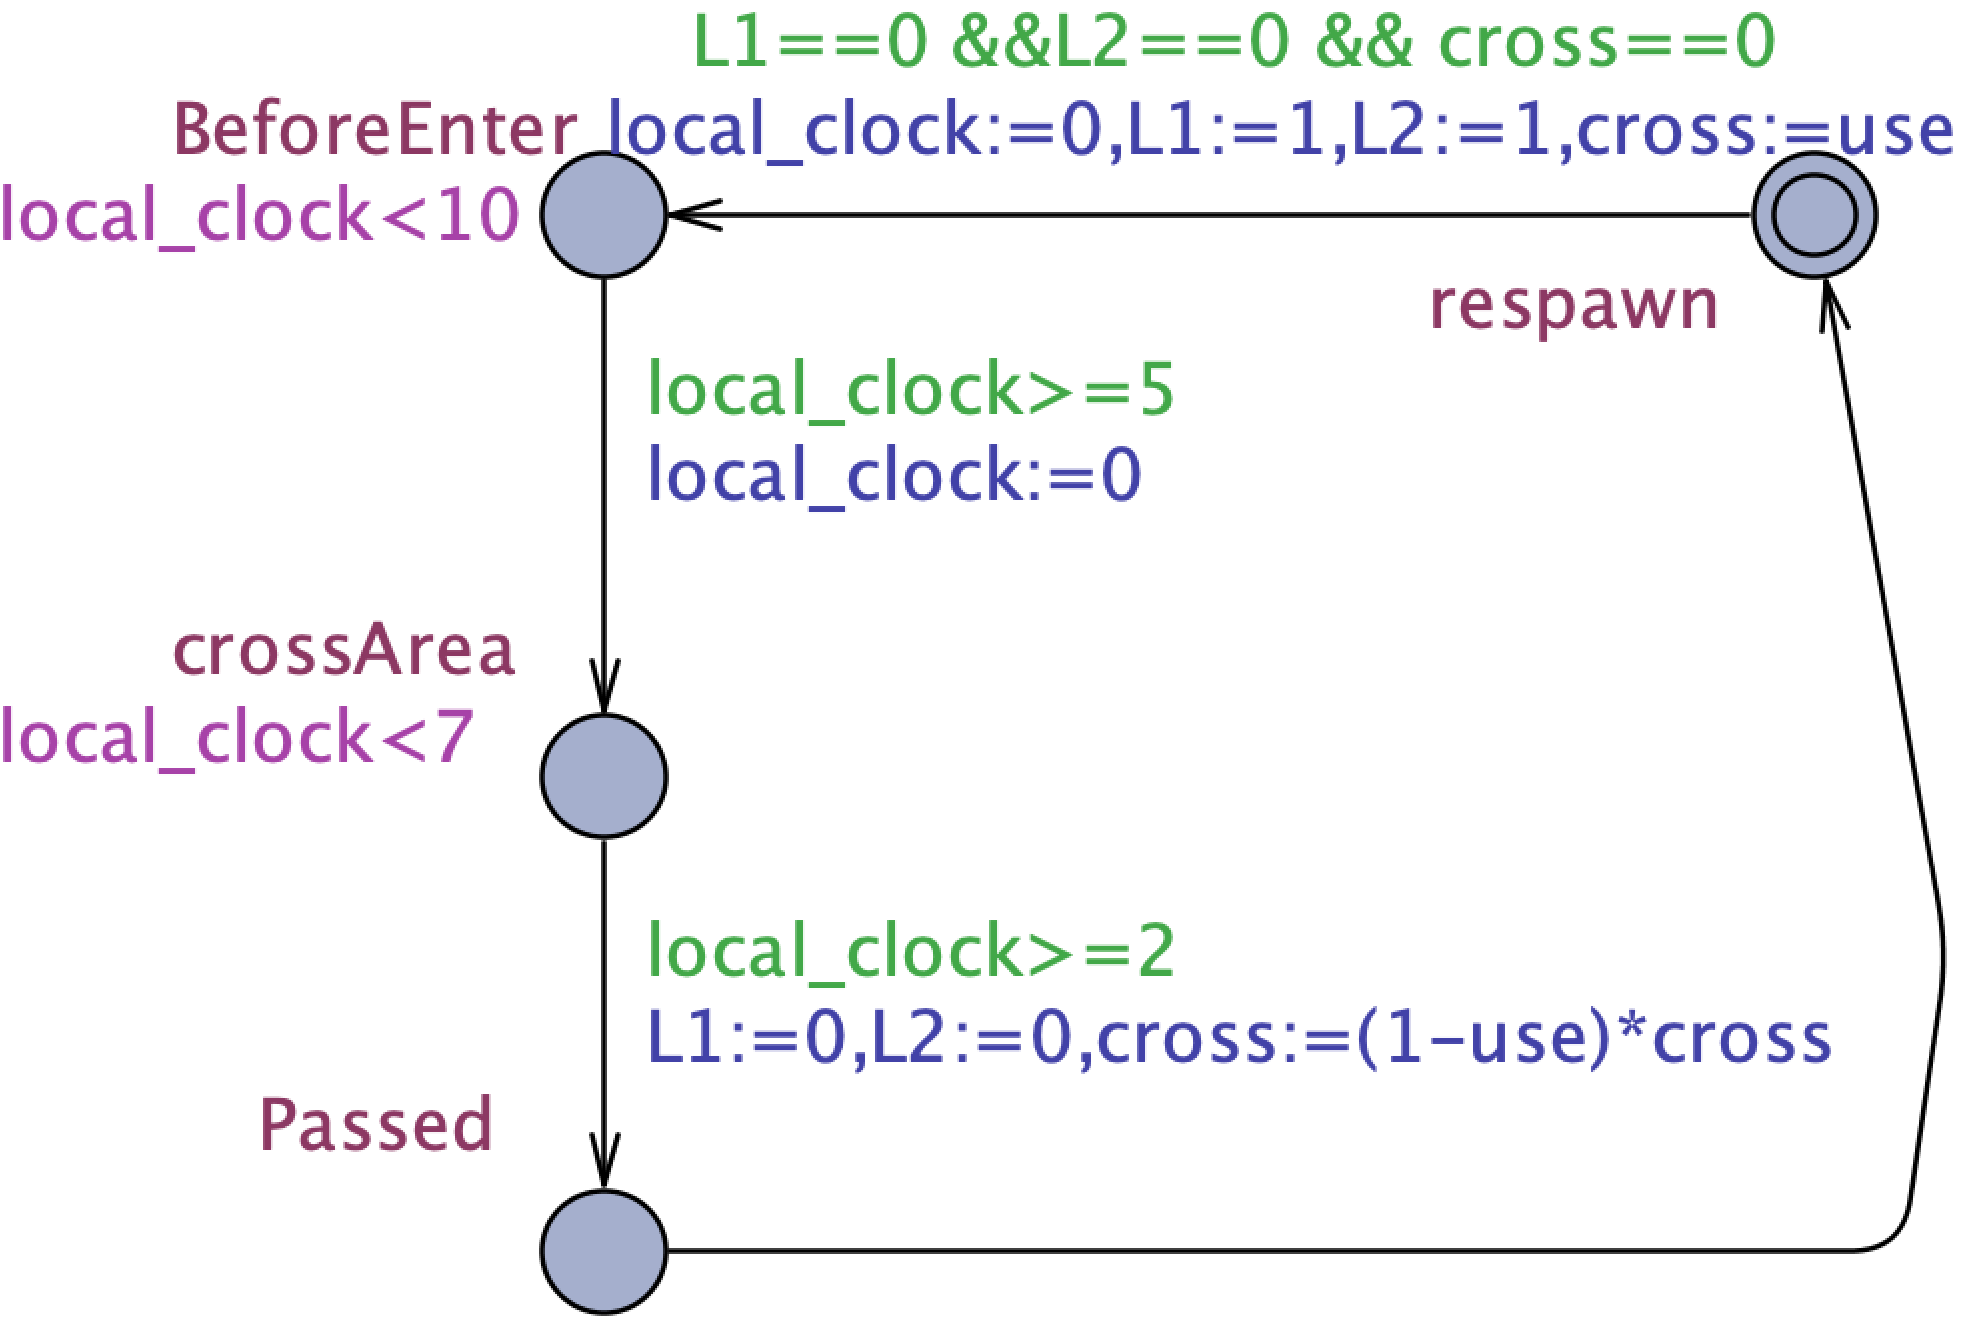
\includegraphics[width=65mm]{SimpleIntersection.png}
	\caption{交差点を通過する車両の時間オートマトン}
	\label{Simple}
	\end{figure}
	\begin{figure}[htbp]
	\centering
	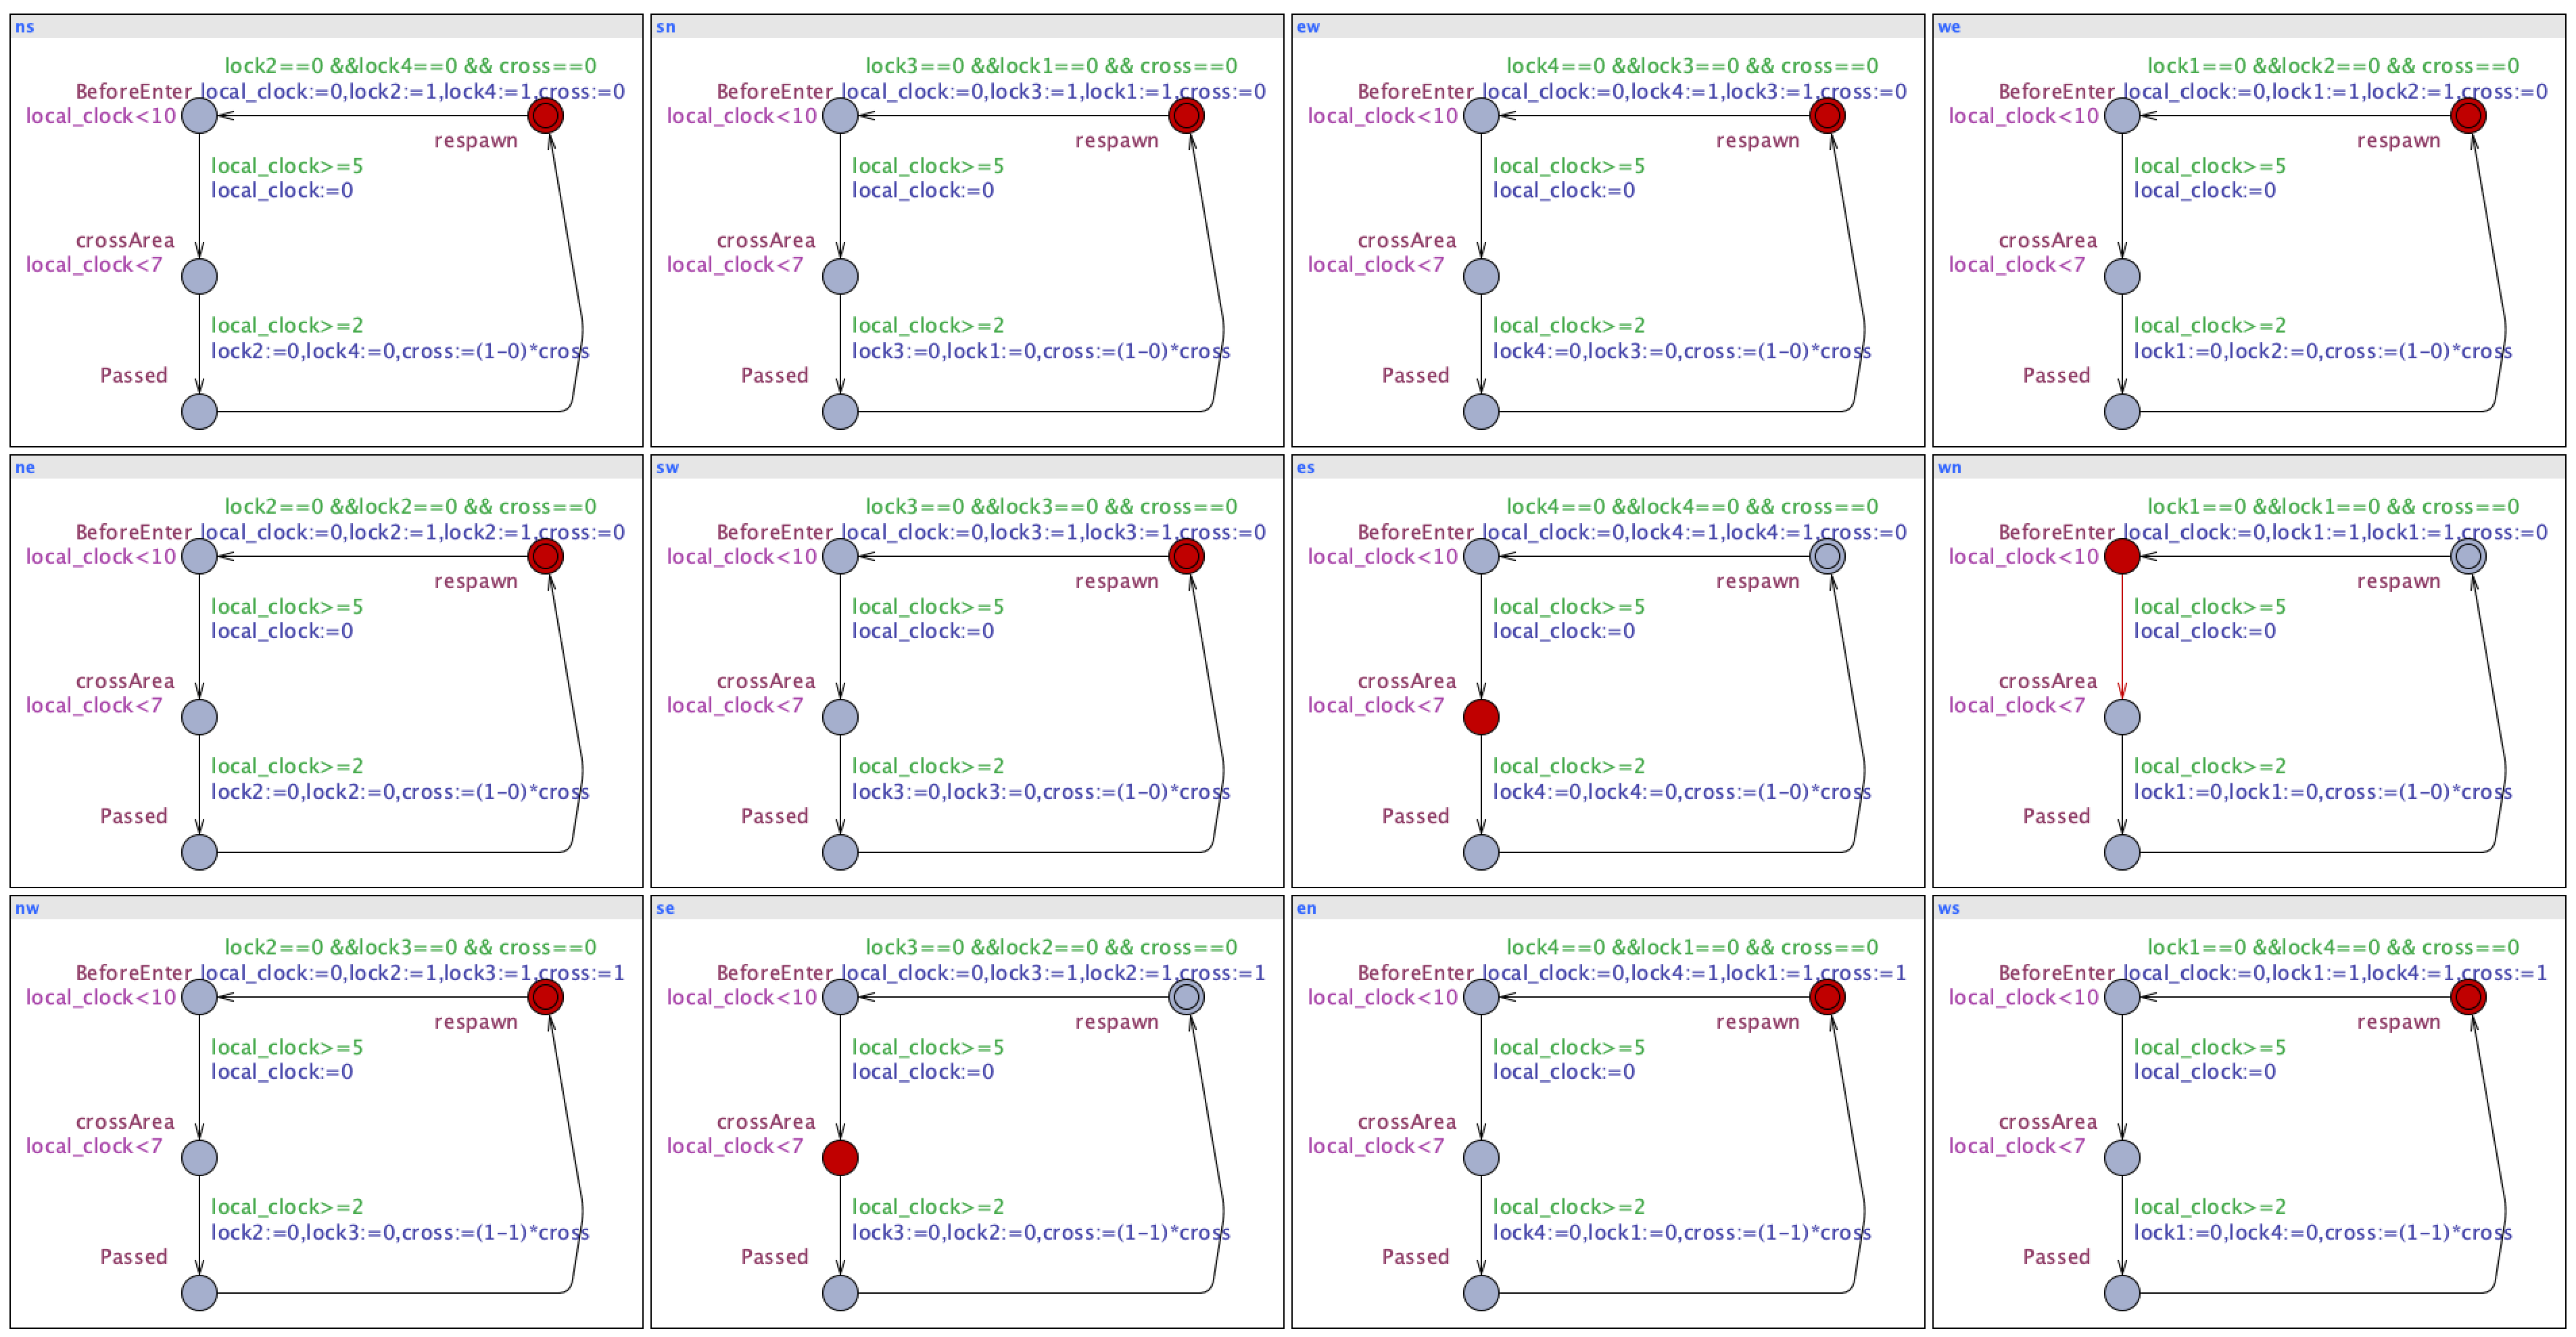
\includegraphics[width=70mm]{SimpleIntersectionSimu.png}
	\caption{交差点を通過する車両の時間オートマトンの合成}
	\label{SimpleS}
	\end{figure}
	\begin{figure}[htbp]
	\centering
	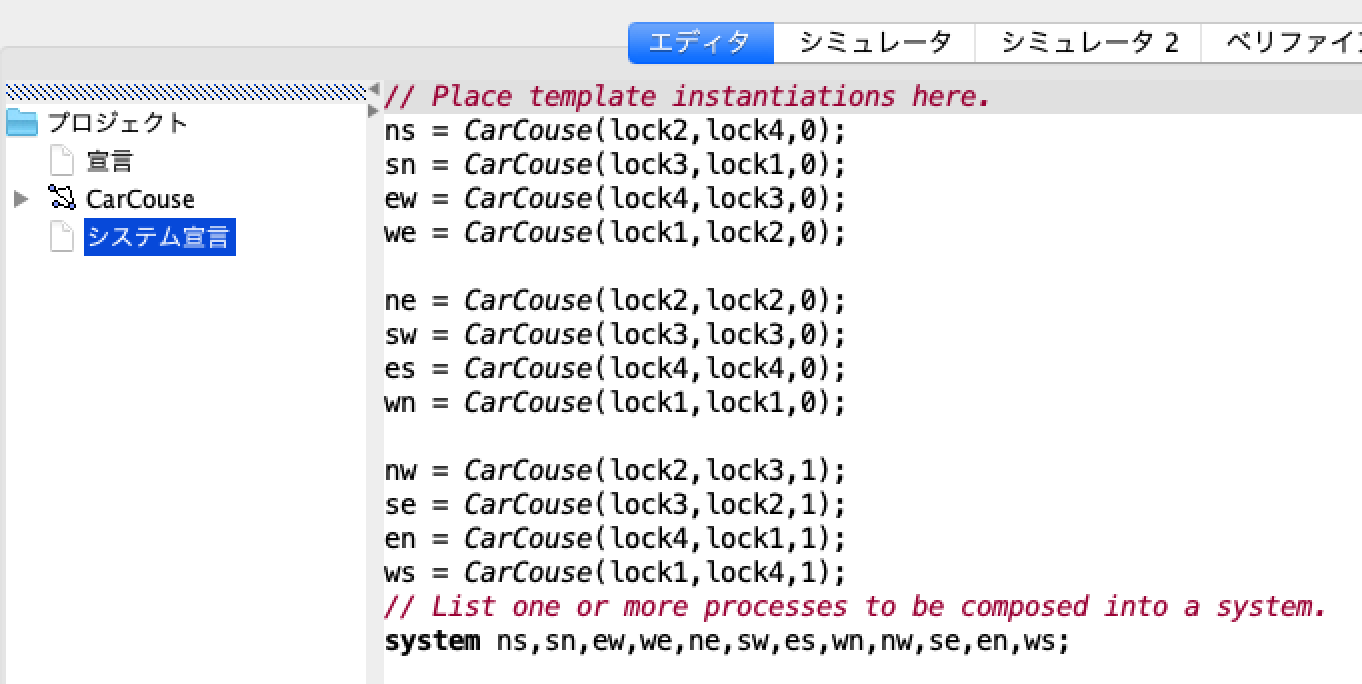
\includegraphics[width=60mm]{SimpleSD.png}
	\caption{12車両のインスタンスの宣言}
	\label{SimpleSD}
	\end{figure}
	\subsubsection{モデル検査}
	デッドロック検証を行った結果を図\ref{SimV}に示す。
	\begin{figure}[htbp]
	\centering
	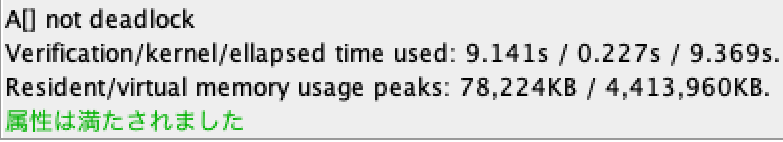
\includegraphics[width=50mm]{SimV.png}
	\caption{12車両で構成される交差点のデッドロック検証結果}
	\label{SimV}
	\end{figure}
	\section{交差点の通過にかかる最小時間の検証}
	本節では,車両全てが交差点を1回通過するのにかかる最小時間について検証を行う。交差点の使用権の取得方法は前節と同仕様の5つ鍵によって管理する。1回だけなので循環するオートマトンではなく一方通行的なオートマトンを作成する(図\ref{minT})。初期状態startから交差点進入前状態BeforeEnterへの遷移可能条件に交差点の使用権の取得として,L1==0かつL2==0かつcross==0を与える。状態BeforeEnterから交差点通過中状態crossAreaへの遷移可能条件とBeforeEnterの状態不変条件で交差点進入前7秒以上10秒未満の間で使用権を獲得しなければならないかを記述し,状態crossAreaから交差点通過後である終了状態finishへの遷移可能条件とcrossAreaの状態不変条件で交差点の通過にかかる時間を記述し,crossAreaからfinishへの状態遷移時に使用権の解除を行う。
	
	最小時間の検証を行う。検証のために大域時間変数gcを宣言する。車両1台のstartからfinishまでプロセスにかかる最小時間は7秒である。車両は全部で12台のため単純に考えると84秒で終わるかと考えられるが,同時通行可能なプロセスもあるため,もう少し少ないと考えられる。例えば図\ref{4L}のように4台同時通行もあり得る。直線が2台ずつ,左折が4台まとめて,右折が1台ずつと考えると,7台分の時間に短縮されると考え,最小時間は49秒と推測し,検証を行う。まず,49秒で本当に全過程が終わる可能性があるかどうかを次の検証式を用いて検査する。
	
	\begin{verbatim}
	
	E<> (gc==49 
		and ns.finish and sn.finish and ew.finish and we.finish 
		and ne.finish and sw.finish and es.finish and wn.finish 
		and nw.finish and se.finish and en.finish and ws.finish)
	
	A[] (gc<49 imply 
		not (ns.finish and sn.finish and ew.finish and we.finish 
		and ne.finish and sw.finish and es.finish and wn.finish 
		and nw.finish and se.finish and en.finish and ws.finish))
	\end{verbatim}
	1つ目の最小時間の可能性である上式は満たされたが,最小時間の最小性はを表す下式は,満たされなかった。すなわち,まだ小さい値を取れる。6台分の時間で検証を引き続き行う。その結果42秒が最小であることが求められた。以下の検証式が成り立つ。その時のルートは図\ref{veriT}の手順だった。
	
	
	\begin{verbatim}
	
	E<> (gc==42 
		and ns.finish and sn.finish and ew.finish and we.finish 
		and ne.finish and sw.finish and es.finish and wn.finish 
		and nw.finish and se.finish and en.finish and ws.finish)
	
	A[] (gc<42 imply 
		not (ns.finish and sn.finish and ew.finish and we.finish 
		and ne.finish and sw.finish and es.finish and wn.finish 
		and nw.finish and se.finish and en.finish and ws.finish))
	\end{verbatim}
	\begin{figure}[htbp]
	\centering
	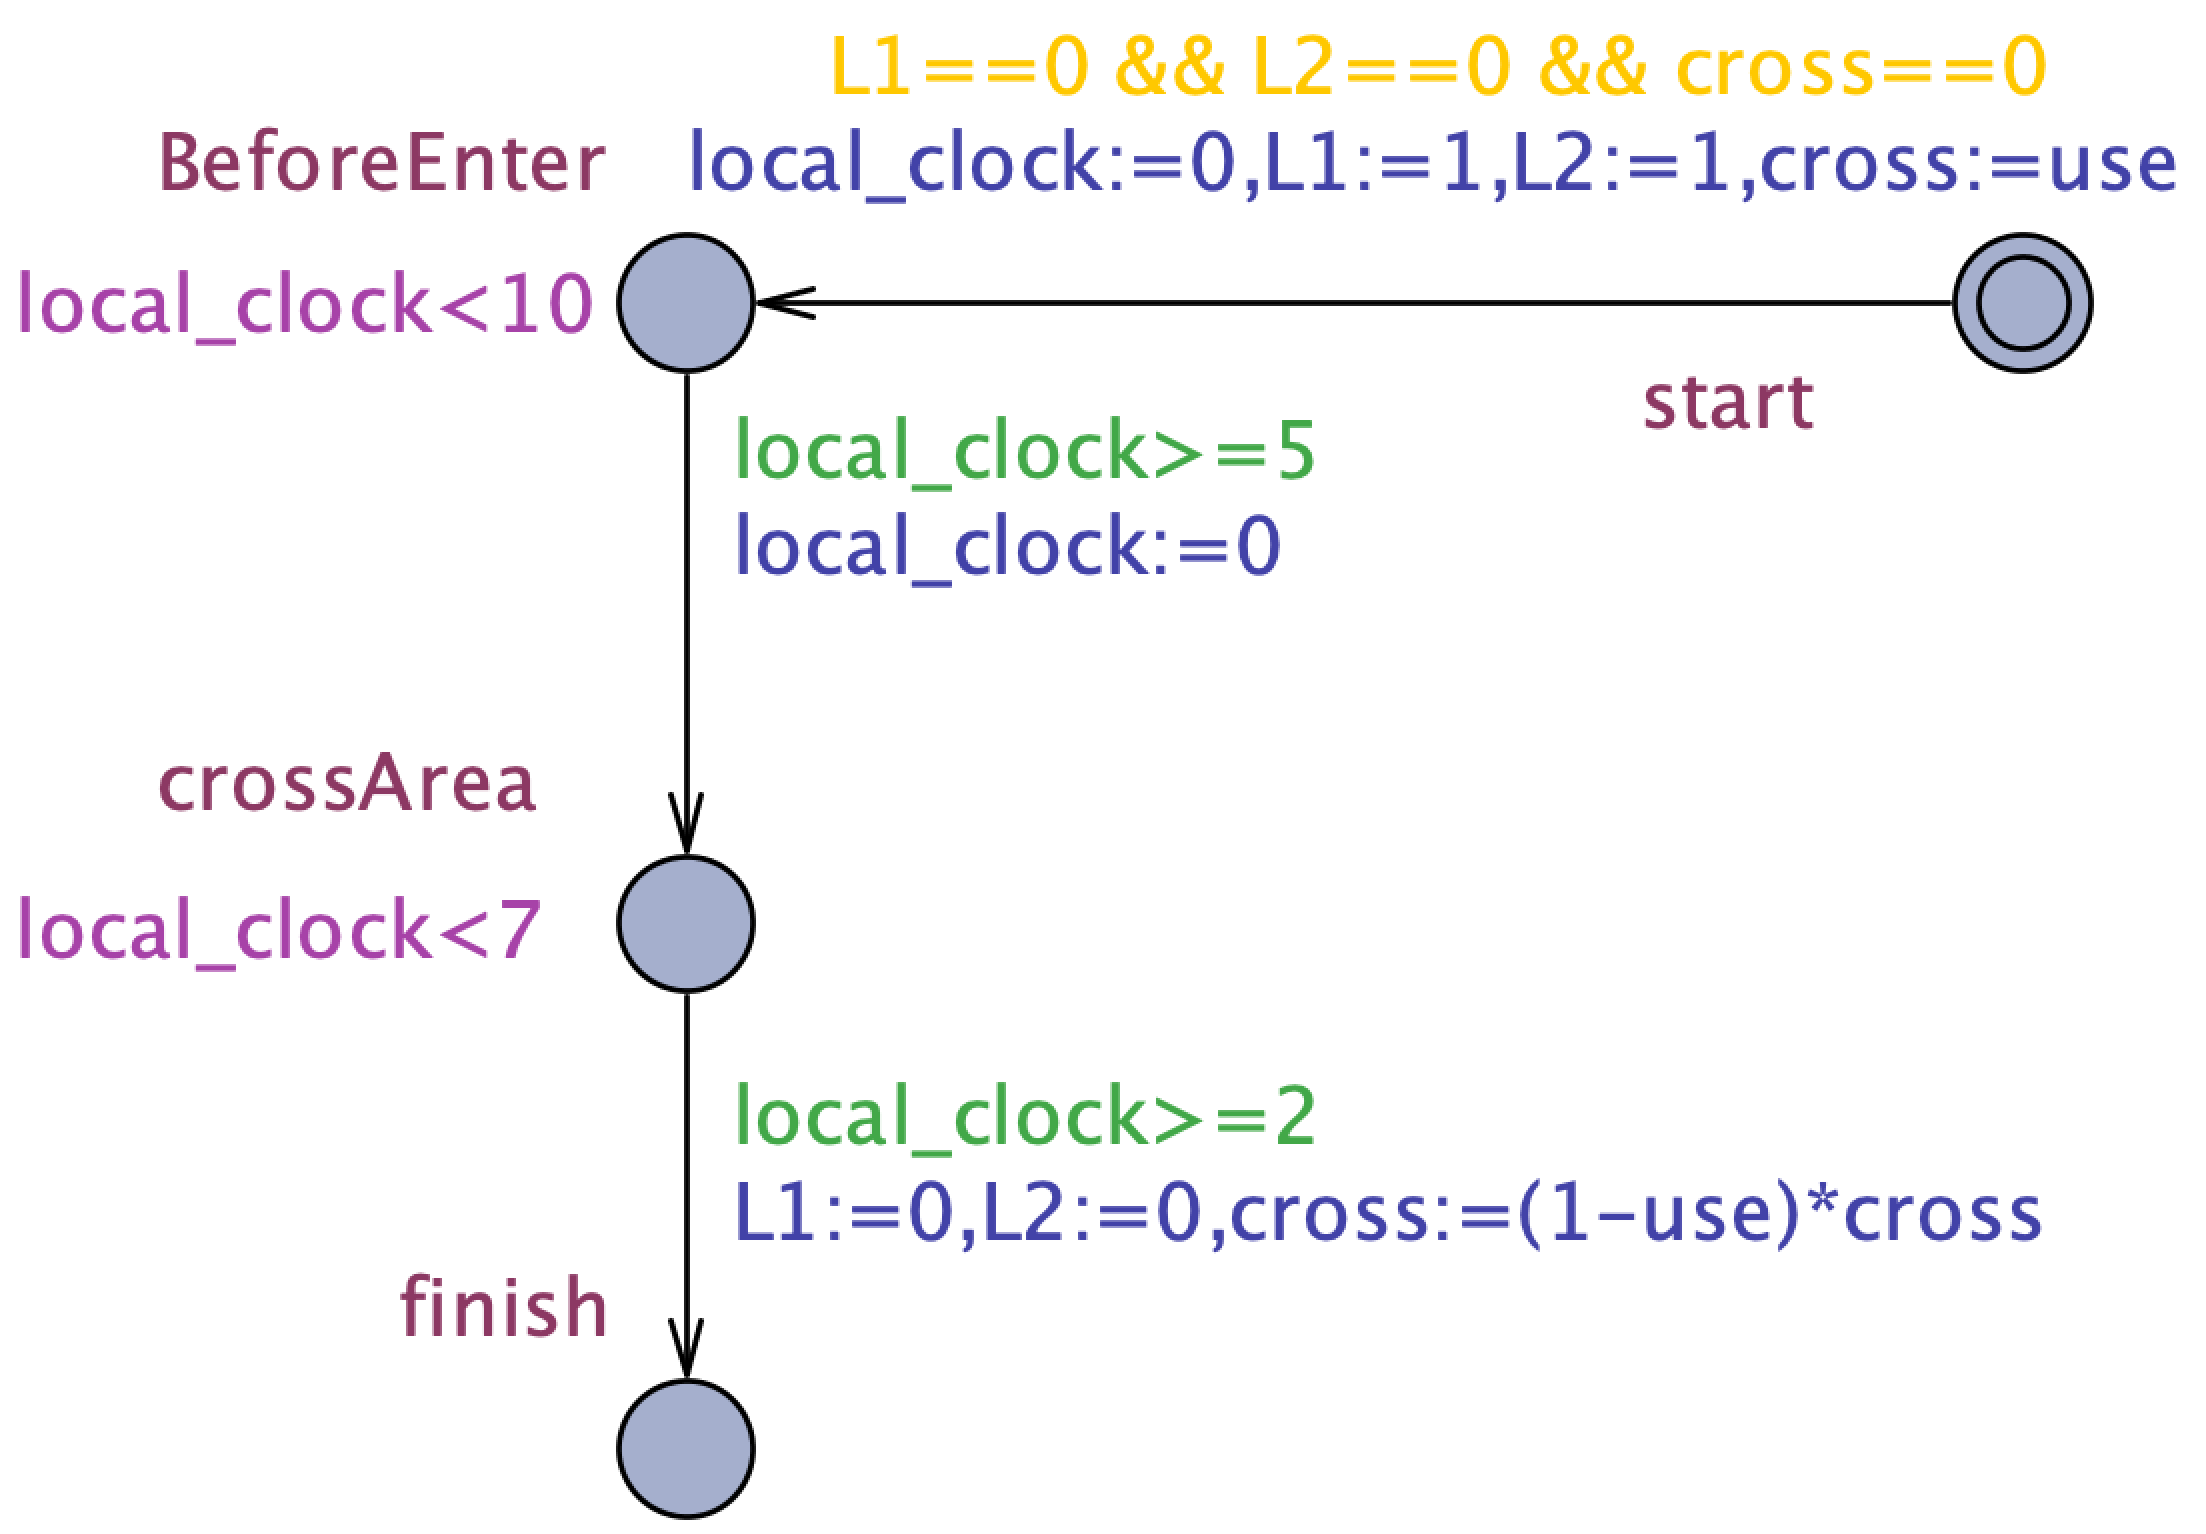
\includegraphics[width=60mm]{minTime.png}
	\caption{交差点を1回通過する時間オートマトン}
	\label{minT}
	\end{figure}
	\begin{figure}[htbp]
	\centering
	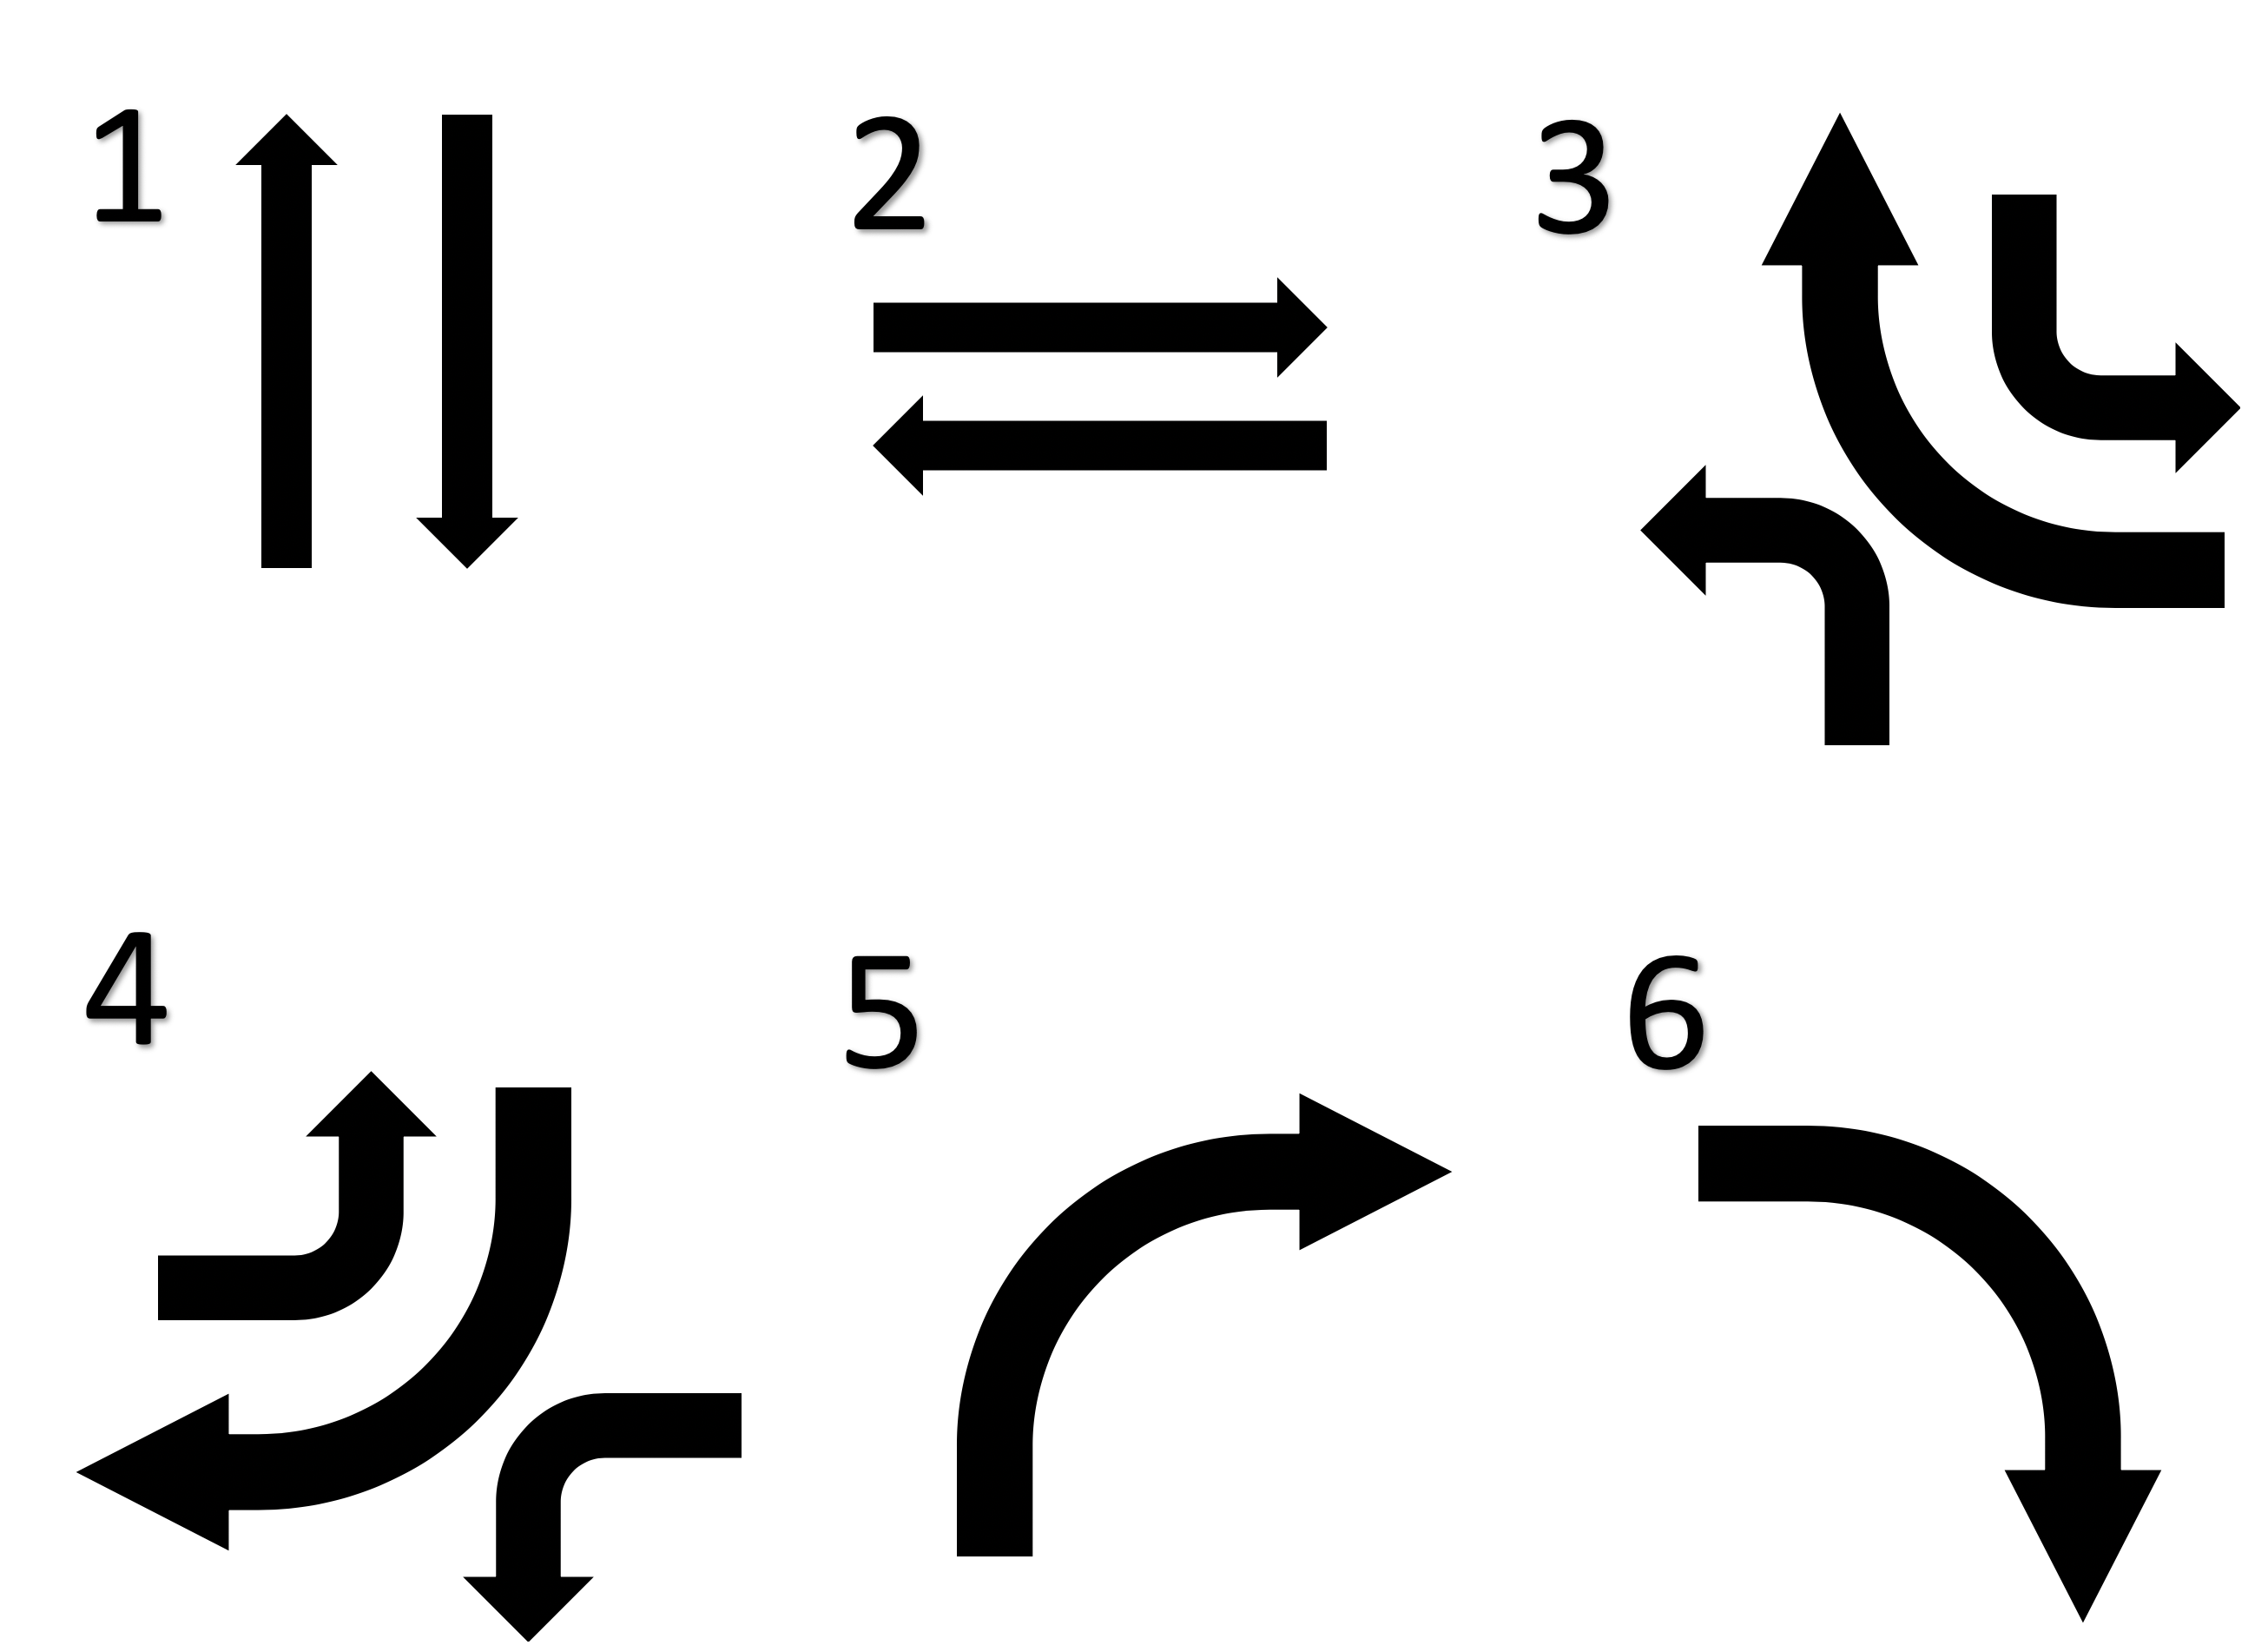
\includegraphics[width=60mm]{veriT.png}
	\caption{最小時間のルート}
	\label{veriT}
	\end{figure}

\section{おわりに}
本研究では,UPPAALを用いた自動運転車群制御アルゴリズムのモデル化と検証の手法を提案した。単一の交差点においては車両の挙動をモデル化し,デッドロックや通過時間を検証することができた。複数の交差点から構成される都市空間のモデルを作成し検証することが今後の課題である。
\begin{thebibliography}{9}
	\bibitem{a1}{長谷川哲夫,田原康之,磯部祥尚, UPPAALによる性能モデル検証ーリアルタイムシステムのモデル化と検証ー, 近代科学社, 2012.}
	\bibitem{Nu}{A. Cimatti, E. M. Clarke, E. Giunchiglia, F. Giunchiglia, M. Pistore, M. Roveri, R. Sebastiani and A. Tacchella,NuSMV 2: An OpenSource Tool for Symbolic Model Checking,In Proceeding of International Conference on Computer-Aided Verification (CAV 2002), pp. 359-364, 2002.}
	\bibitem{n2}{NuSMV home page, \verb$http://nusmv.fbk.eu$}
	\bibitem{s1}{G.J. Holzmann, The SPIN Model Checker: Primer and Reference Manual, Addison-Wesley, 2003.}
	\bibitem{s2}{Spin - Formal Verification, \verb$http://spinroot.com$}
	\bibitem{u1}{Uppaal in a Nutshell. Kim G. Larsen, Paul Pettersson and Wang Yi. In Springer International Journal of Software Tools for Technology Transfer 1(1+2), 1997.}
	\bibitem{u2}{UPPAAL, \verb$http://www.uppaal.org$}
	\bibitem{u3}{Timed Automata: Semantics, Algorithms and Tools, Johan Bengtsson and Wang Yi. In Lecture Notes on Concurrency and Petri Nets. W. Reisig and G. Rozenberg (eds.), LNCS 3098, Springer-Verlag, 2004.}
	\bibitem{a9}{綿引健二, 石川冬樹, 平石邦彦, 時間, 資源の制約をもつビジネスプロセスの形式検証, 電子情報通信学会論文誌 D, 96(8):1878-1891, 2013.}
\end{thebibliography}
\end{document}